\documentclass[10pt]{article}
\usepackage{../../local}
\usepackage{listings}
\lstdefinestyle{tt}{basicstyle=\small\ttfamily,keywordstyle=\bfseries,language=[LaTeX]{TeX}}



\newcommand{\classcode}{CS 170}
\newcommand{\classname}{Efficient Algorithms and Intractable Problems}
\renewcommand{\maketitle}{%
\hrule height4pt
\large{Eric Du \hfill \classcode}
\newline
\large{Notes} \Large{\hfill \classname \hfill} \large{\today}
\hrule height4pt \vskip .7em
\normalsize
}
\linespread{1.1}

\newcommand{\pre}{\mathrm{pre}}
\newcommand{\prev}{\mathrm{prev}}
\newcommand{\post}{\mathrm{post}}
\newcommand{\dist}{\mathrm{dist}}
\newcommand{\cost}{\mathrm{cost}}
\newcommand{\size}{\mathrm{size}}
\newcommand{\capacity}{\mathrm{capacity}}

\newcommand{\question}[1]{\textcolor{red}{#1}}
\newcommand{\answer}[1]{\textcolor{green!80!black!}{#1}}
\renewcommand{\comment}[1]{\textcolor{blue!50}{#1}}
\begin{document}
	\maketitle
	\section{Graphs}
	Formal definition of undirected graphs:
	\begin{itemize}
		\item Called $G(V, E)$.
		\item has a set $V$ of vertices, and $E$ of edges.
		\item Edges are denoted as a pair of vertices $\{v_i, v_j\}$, and undirected mean that each 
			pair of $\{v_i, v_j\}$ is unique.
			\begin{itemize}
				\item e.g. Facebook friendship graphs, where the friendship must be mutual. (Has nearly 3 billion
					nodes, and each node has 330 vertices)
			\end{itemize}
		\item Directed graph is denoted in the same way, except that $\{v_i, v_j\}$ means 
			specifically that $v_i \to v_j$.
	\end{itemize}

	\subsection{Size of Graphs}
	\begin{itemize}
		\item Generally denoted as the number of vertices (denoted by $n$) and the number of edges 
			(denoted by $m$).
		\item $m$ can be at most $n^2$, in the case that every vertex is connected to every other vertex 
			(in which case we have $n(n-1)$ edges)
		\item Degree: the number of edges that a vertex has. With directed graphs, we can specify in-degrees
			and out-degrees.
	\end{itemize}

	\subsection{Representing Graphs}
	\begin{itemize}
		\item Represented either as an adjacency matrix or an adjacency list.  
			\begin{itemize}
				\item Adjacency matrix: have the vertices listed out on both row and column, put a 1 if 
					$\{v_i, v_j\}$ are connected on our graph.
				\item Adjacency list: List of length $n$, and each cell is a linked list that points 
					to all the neighbours of $v_i$.
			\end{itemize}
		\item There are tradeoffs for both ways:
			\begin{center}
				\begin{tabular}{c|c|c}
			& 	\textbf{Adjacency Matrix} & \textbf{Adjacency List}\\
			\hline
					Storage Size  & $O(n^2)$  & $O(n + m)$\\
				Checking whether $(u, v) \in E$ & $O(1)$ & $O(\deg(u))$\\
				Enumerate all of $u$'s neighbours &  $O(n)$ & $O(\deg(u))$
				\end{tabular}
			\end{center} 
		\item We will work with adjacency lists, since the storage size for adjacency matrices get
			too large too quickly. 
	\end{itemize}
	\subsection{Graph Connectedness}
	\begin{itemize}
		\item We first have to solve the problem of graph traversal. Our approach will use ``string and chalk,''
			so we mark when we've reached a dead end and the ``string'' will allow us to backtrack. 
		\item Algorithm description:

\begin{lstlisting}[style=tt]
def explore():
	visited[u] = true

	For all edges of $u$: if visited[v] = false then run explore(v)
\end{lstlisting}
		\item Explore guarantees that all the vertices that are visited by explore have a path from $u$ to 
			that vertex, and vice versa.
			\begin{itemize}
				\item We prove the other direction: if there's a path, then that node is visited.

					Assume that this is false: assume $\exists v$ that hasn't been explored but there is 
					a path from $u$ to $v$. Instead of looking at $u$ to $v$, we look at the path 
					from $u$ to $v_k$, the first node along the path from $u$ to $v$ that is unexplored. 
					This means that the algorithm reached $v_{k - 1}$, then failed to explore $v$.

					This is a contradiction, since explore must have been called on $v_{k-1}$, but failed to 
					recurse down $v_k$. 
			\end{itemize}
	\end{itemize}

	\subsection{Depth First Search (DFS)}
	Essentially calling explore, except it does it recursively on all the remaining nodes that haven't 
	been visited yet.
	\begin{itemize}
		\item We can also use DFS to find the connected components of a graph! When we explore with DFS, we are 
			implicitly exploring connected components, this uses the transitive fact of the \texttt{explore()}
			function.
		\item The edges that are visited by DFS are categorized into tree edges and back edges. Tree 
			edges are edges that are used when the algorithm runs, and back edges are ones that exist within 
			the original graph but aren't used. 
		\item There's a third class called a \textit{cross edges}, but they cannot exist for an undirected graph.
			\begin{itemize}
				\item The proof is by contradiction: imagine that it did exist, then DFS would have called
					explore on that ancestor; but it can't possibly have since $u$ and $v$ do not 
					exist in the same branch.
				\item They \textit{can} exist in a directed graph, since we only traverse through out 
					edges (so there can be an in-edge that never gets traversed).
			\end{itemize}
	\end{itemize}	

	\subsubsection{DFS Runtime}
	\texttt{Explore()} is called only once per node, and the runtime for each node for explore is 
	proportional to $\deg(u)$, so the total is:
	\[
		\sum_{u \in V} O(1 + \deg(u)) = O(n + m)
	\] 

	\subsection{DFS for Directed Graphs}
	It's the same principle, our explore still only runs recursively on unvisited neighbours, but we need 
	to also keep track of the amount of time at which we start and finish processing that node.
	\begin{itemize}
		\item Every time we enter a node, we stamp it with the time of the start clock. When we come 
			out, we stamp again with the end clock. Every time we progress the clock, we increment it by 1.
		\item The point of the clock will be revealed later on in future lectures. 
		\item The edges we keep track of here are forward, back and cross edges. Forward means we go 
			down the tree from ancestor to descendant (not its immediate child), back means we go backwards 
			(can be immediate) and cross edges are defined exactly as before.
	\end{itemize}
	The edges (pre, post, cross) are useful in determining properties of the graph $G$. 
	\begin{itemize}
		\item Cross edges can only go from a later point in one branch to earlier than the other branch
			and not the other way around, due to the way that DFS executes depth-first.
		\item Suppose $(u, v) \in E$ is a tree edge. Then, we know that $\pre(u) < \pre(v)$ (since $u$ is 
			hit first), and $\post(u) < \post(v)$. 
		\item Suppose that $(u,v)\in E$ is a back edge. Then, we have $\pre(v) < \pre(u) < \post(u) < \post(v)$.
	\end{itemize}

	\section{Strongly Connected Graphs}
	Recall that we saw earlier that DFS basically just calls explore repeatedly, to find all the vertices 
	reachable from a vertex $u$. We also introduced two clocks, where when we first visit a node 
	we stamp it with the start clock, and that vertex will have a $\pre(u)$ quantity that stores its value, 
	then increments clock. When we leave the vertex, we stamp again with a $\post(u)$. 

	\begin{itemize}
		\item For cross edges (the only thing we didn't finish last time), we have $\pre(v) < \post(v) <
			\pre(u) < \post(u)$ (we get to $v$ and finish exploring $v$ before we ever touch $u$).
		\item As a recap:
			\begin{center}
				\begin{tabular}{c|c}
					Edge type & Relation\\
					\hline
					Tree edge & $\pre(u)< \pre(v) < \post(v) < \post(u)$\\
					Back edge & $\pre(v) < \pre(u) < \post(u) < \post(v)$\\
					Cross edge & $\pre(v) < \post(v) < \pre(u) < \post(u)$
				\end{tabular}
			\end{center}
	\end{itemize}


	\subsection{Topological Sort} 
	\begin{itemize}
		\item The process of finding an ordering of vertices so that no edges go backwards. This is used 
			in software package loading, to make sure that things aren't being and that are being downloaded
			in the chronological order. 
		\item Mathematically, if $u$ comes before $v$ in the ordering, then there is no edge $(v, u)$. 
		\item Two types of special nodes: \textbf{sources} and \textbf{sinks}
			\begin{itemize}
				\item \textbf{Source:} A node that has no incoming edges and has only outgoing edges. 
				\item \textbf{Sink:} A node that has no outgoing edges and only has incoming edges
			\end{itemize}
		\item Note that a node with no edge at all is considered both a source and a sink.
	\end{itemize}
	
	\subsection{DAGs}
	\begin{itemize}
		\item Called a directed acyclic graph, or basically just a graph without any directed cycles. If 
			we have a cycle, then we can't toplogically sort. 
		\item We will find that if we run DFS on a graph, it is a DAG iff it has no back edges.
			We prove that if we have a back edge, then it cannot be a DAG: since they go from something 
			that's already been visited to something that's been visited earlier, then we have already 
			found a cycle. 

			Now we prove that if we don't have a DAG (i,e, has a cycle) , then it has a back edge. Since DFS
			visits every vertex in 
			a graph, it will eventually enter our cycle at some $v_i$. Then, it will traverse through the cycle
			until it visits all the nodes and eventually gets to $v_k$, the node right before it comes back to 
			$v_i$. 
			Then, $v_k \to v_i$ will become a back edge, since it was visited earlier in the graph.
		\item Back edges are really special! Recall that we only have a back edge when $\post(u) < \post(v)$, 
			since the other edges have $\post(v) < \post(u)$. We then conclude that if we have a DAG, then 
			it has the property that $\post(v) < \post(u)$ (since it can't have back edges). 
			
			\question{Does 
				the logic work the other way around? Does 
			this mean that if $\post(u) < \post(v)$ then we have a DAG?}

			\answer{Not necessarily. Just because $\post(v) > \post(u)$ doesn't necessarily imply that a 
			back edge exists.}
		\item Our algorithm for topological sort: do a DFS on graph $G$, then enumerate all $v \in V$ in 
			the decreasing order of $\post(v)$. 
	\end{itemize}

	\subsection{Strongly Connected Components}
	
	\begin{itemize}
		\item To find DAGs on undirected graphs we can run DFS on them, but what about directed graphs? 
		\item \textbf{Definition:} Vertices $u$ and $v$ are strongly connected if there is a path from $u$ to 
			$v$ and there is also a path from $v$ to $u$. 
		\item A graph is \textit{strongly connected} when all of its vertices are strongly connected.
		\item Generally, we partition a graph into \textit{strongly connected components}, since it's very rare
			that the 
			entire graph is strongly connected.
		\item Strong connectivity is an example of an equivalence relationship, since it satisfies all 
			the properties: reflexive, symmetric and transitive.
			\begin{itemize}
				\item Every vertex is strongly connected to itself
				\item If $A$ is strongly connected to $B$, then $B$ is strongly connected to $A$. 
				\item If $A$ is strongly connected to $B$ and $B$ is strongly connected to $C$, then $A$ 
					is strongly connected to $C$.
			\end{itemize}
		\item If we flip all the edge (i.e. reverse the direction), the strongly connected components don't 
			change at all! 
		\item We can then divide this into a \textit{meta graph}, where we group the graph by strongly 
			connected components (try to be as general as possible when you do this).
			\begin{itemize}
				\item The meta graph can't have cycles! Had a cycle existed, then it would imply that vertices 
					from one strongly connected component can reach vertices of another, and vice versa!
				\item Therefore, the meta graph \textit{must} be a DAG.
			\end{itemize}
		\item Why care about SCC? It is useful in many different fields, since SCCs naturally imply 
			a strong equivalence of objects in a graph.
	\end{itemize}
	\subsection{Finding SCCs}
	\begin{itemize}
		\item \textbf{Attempt 1:} Consider all possible decompositions and check (BAD!)
		\item \textbf{Attempt 2:} Consider pairs of nodes, then run explore to see if they reach the other. 
			(ALSO BAD!)
		\item There exists an algorithm that runs this in $O(n + m)$ time, where we have to run DFS (smartly) 
			only twice!
	\end{itemize}
	\subsubsection{More Properties of SCCs}
	\begin{itemize}
		\item It actually matters where we start our DFS, since sometimes we can't exit the particular 
			connected component. Specifically, if the node is part of a source in the meta graph, then 
			it will visit many nodes, whereas if the node is a sink then we never exit that particular connected
			component.
		\item The ``right'' place to start the DFS is in the \textbf{sink of the meta graph!} The key 
			thing is that we shouldn't exit that connected component, so running \texttt{explore()} on 
			any vertex within this CC will give us the whole SCC.
		\item \textbf{Idea:} Do the topological sort on the meta graph, then run DFS on the sinks of 
			the meta graph.
		\item Suppose we run DFS on a graph $G$. Let $C$ and $C'$ be two connected components such that $C \to 
			C'$ in the meta graph. Then, $\max(\post(v \in C)) > \max(\post(u \in C'))$.

			\textit{Proof:} Split into cases, based on where in the graph we started:

			Case 1: Suppose DFS visited $C$ first ($u \in C$ is the first node visited by DFS. Then, 
			DFS will explore $C'$ first before finishing its exploration of $C$. This means that DFS finishes
			$C'$ before finishing $C$, meaning that $\max(\post(v \in C)) > \max(\post(u \in C'))$.

			Case 2: Suppose DFS visited $C'$ first. Then, we will never visit $C$ since there is no directed
			edge between $C' \to C$. Therefore, the post of $C'$ stops before DFS even reaches $C$, Hence, 
			we have $\max(\post(u \in C')) < \max(\post(v \in C))$. 
		\item Immediate corollary of this: Suppose we ran DFS on a graph $G$. The highest $\post(v)$ belongs 
			to a node $v$ that is in the source SCC of the meta graph!
			\begin{itemize}
				\item Imagine $\max(\post(C))$ is not the largest $\post(v)$ value. Then, this means that 
					there exists another $C''$ whose $\post(C'')$ is larger than that of $C$!
			\end{itemize}
		\item So now we have a way of finding the source of the vertices in $C$, but we want to start from 
			sinks, so we \textbf{flip the edges, then run DFS!} The only difference betweeh $G$ and $G^R$ (the 
			reversed graph) is the direction of the edges; the connected components remain the same.

			\question{Instead of flipping edges, why not run the algorithm from the minimum post value 
			instead?}

			\answer{Because the minimum isn't guaranteed to be a SCC in the same way the max is.}
	\end{itemize}

	\subsection{The Algorithm}
	\begin{itemize}
		\item Compute $G^R$.
		\item Run DFS on $G^R$.
		\item Store the post numbers of this DFS in array called post-r 
		\item Run DFS on $G$, but explore unvisited nodes in \textit{decreasing} order of post-r. For every 
			DFS we run, we find a new SCC.
	\end{itemize}
	\section{Paths in Graphs}

	\subsection{Single Source Shortest Path (SSSP)}
	\begin{itemize}
		\item We want to compute the distances from a source $s \in V$ to other nodes in $V$. 
		\item We don't use DFS here because DFS might explore much longer paths first, so it might be very 
			inefficient.
		\item Solution: use \textbf{Breadth-First Search (BFS)}
			\begin{itemize}
				\item Analogous to a bird's eye perspective, where we explore successively outward in 
					``neighbourhoods.''
				\item Start at exploring from distance 1, then when everything at distance 1 is explored, 
					continue to explore at distance 2, etc. 
			\end{itemize}
		\item The type of BFS that we use depends a lot on what kind of graph we're dealing with:
			\begin{itemize}
				\item Unweighted graphs: Ordinary BFS works
				\item Positive Weights: Dijkstra's algorithm
				\item Negative Weights allowed: Bellman-Ford Algorithm
			\end{itemize}
		\item Going down this list makes the graph more general, but they are less efficient than the ones 
			above. 

			\question{Would a more correct statement be that BFS works if all the edges have the same weight?}
	\end{itemize}

	\subsection{Breadth First Search (BFS)}
	\begin{itemize}
		\item Start at $s$, and add all the neighbours of $s$ to a queue. For every vertex in 
			the queue, we visit all the unvisited nodes from that vertex, and add it to the queue. Repeat
			until all nodes have been visited.
	\end{itemize}

	\subsubsection{Runtime of BFS}
	\begin{itemize}
		\item 	We enqueue and deque every node exactly once if the node is connected, otherwise we don't do it 
			at all. This takes $O(1)$ time. 
		\item Once an item is dequeued, we need to check all the neighbours of a graph, costing $O(\deg(u))$ 
			time.
		\item In total, our runtime is:
			\[
				\sum_{u \in V} O(1 + \deg(u)) = O(n + m)
			\] 
			This is the same runtime as DFS, which is not a coincidence! DFS and BFS are actually related, 
			except the queue is replaced by a stack.
		\item We didn't implement it as a stack in lecture, but the idea is the same.
	\end{itemize}

	\subsection{Weighted Graphs}
	\begin{itemize}
		\item BFS doesn't work here because it ignores the weights of the graph. It is possible that a graph 
			ends up being shorter but goes through more nodes, a possibility that BFS doesn't catch.
		\item \textbf{Useful Fact:} Any sub path of a shortest path is also a shortest path. This is rather 
			obvious.
		\item So what we should think about is that to build the shortest path, we build the shortest path from 
			other, shotest paths but add in the shortest edge. This guarantees that our shortest path 
			remains the shortest.
	\end{itemize}

	\subsection{Dijkstra's Algorithm}
	\begin{itemize}
		\item Let $K$ denote the set of ``known'' nodes where the length of shortest path is computed. To 
			determine node we should add to $K$, we should select the vertex that gives the smallest 
			$\dist(s, u) + \ell(u, v)$. Visually:
			\begin{center}
				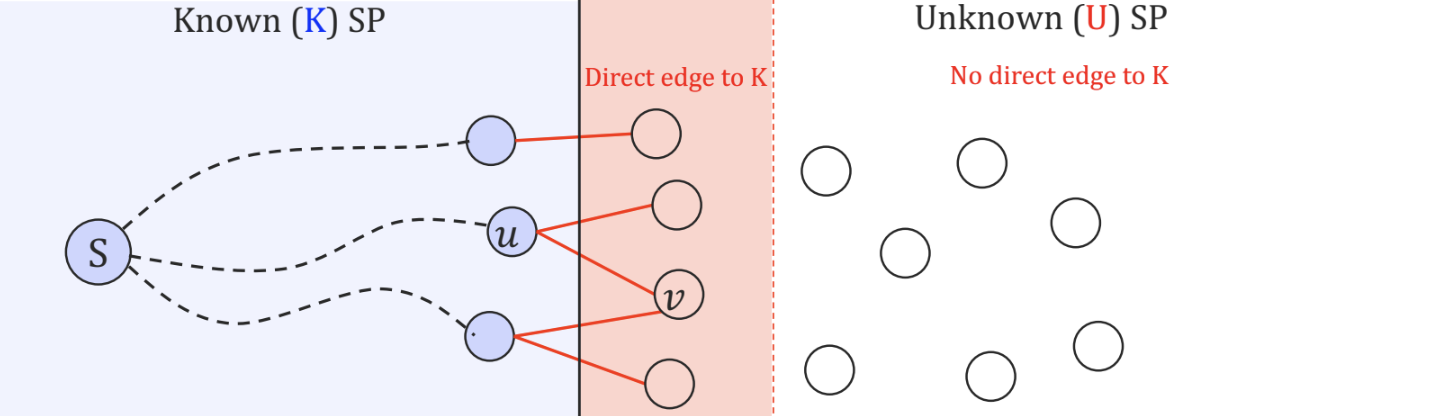
\includegraphics[scale=0.5]{dijkstra.png}
			\end{center}
		\item The red region is the set of nodes that we look at.
		\item We don't need to recompute all distances at every iteration - instead we can just store 
			the distances as we go along. Initial overestimates are fine, since eventually we will explore 
			the shortest path, and its distance will eventually be updated. 
		\item If we find a shorter path later on, we can update $\dist(s, u)$ to reflect that.
		\item If we want to find the shortest path from $S$, then we can add a new variable that stores 
			the previous node in the sequence from $S$ to $u$. Therefore, when we want to find the 
			shortest path, then we are continually looking backward until we get back to $S$. 
	\end{itemize}

	\subsubsection{Runtime of Dijkstra's}
	\begin{itemize}
		\item The runtime of Dijkstra's depends on the kind of data structure we used to keep track 
			of the distances:
			\begin{center}
				\begin{tabular}{c|c|c|c|c}
					\textbf{Implementation} & \textbf{Insert} & \textbf{Delete Min} & 
					\textbf{Decrease Key} & \textbf{Runtime}\\
					\hline 
					Array & $O(1)$ & $O(n)$ & $O(1)$ & $O(n^2 + m) = O(n^2)$\\
					Binary Heap & $O(\log n)$ & $O(\log n)$ & $O(\log n)$ & $O((n + m) \log n)$\\
					Fibonacci Heap & $O(1)$ & $O(\log n)$ & $O(1)$ & $O(n \log n + m)$
				\end{tabular}
			\end{center}
		\item The best known runtime of Dijkstra's algorithm is $O(n \log \log n + m)$.
		\item At the end of the day, this is slower than DFS, by the $\log n$ term.
	\end{itemize}
	
	\subsection{Negative Weights: Bellman-Ford Algorithm}
	\begin{itemize}
		\item Sometimes, having negative weights is possible, for instance when traversing an edge is more 
			beneficial to you in some way.
		\item Shortest paths don't really make sense if a cycle has negative length (since then we'd be 
			infinitely descending) 
		\item All we need to do is modify Dijkstra's update function!
			\begin{itemize}
				\item Call an update ``safe'' if $\dist(w)$ is an overestimate of the true shortest path 
					between $s$ and $w$. In other words, $\dist(w) \ge d(s, w)$ for all $w \in V$. 
			\end{itemize}
	\end{itemize}

	\question{see lectures for Bellman-Ford}

	\section{Greedy Algorithms}

	\begin{itemize}
		\item Are algorithms that build their solution piece by piece, and always takes the piece that 
			offers the \textbf{most obvious and immediate benefit}.
		\item Some applications of where Greedy algorithms do work: Scheduling, satisfiability, Huffman Coding
			MSTs. 
	\end{itemize}
	\subsection{Scheduling}
	\begin{itemize}
		\item Input: collection of jobs specified by their time intervals $[s_1, e_1], \dots, [s_n, e_n]$. We
			want to find the largest subset of jobs that have no time conflicts.
		\item To do this, after choosing an interval, we'd want to choose the next interval that 
			has the \textit{earliest end time}. Jobs that finish earlier give us more opportunities to 
			slot in more jobs later in the day. 
			\begin{itemize}
				\item This is not achieved by selecting the shortest job, because it does not give us freedom 
					in where $s_i$ and $e_i$ are. 
				\item This is also not achieved by selecting the earliest job, since we don't know where $e_i$
					is. 
			\end{itemize}
		\item So our code is as follows:

			While set of intervals is not empty: \\
			Add interval $j$ with the earliest finish time $e_j$. \\
			Remove any conflicted interval $i$ from the set, i.e. $[s_j, e_j] \cap [s_i, e_i] \neq 
				\emptyset$.
		\item The runtime of this algorithm is $O(n)$ if the intervals are already sorted by the end time,
				otherwise, we'd need $O(n \log n)$ time since we'd need to sort the intervals first.
		\item To show that the greedy algorithm works, we need to show that this algorithm doesn't rule out 
			an optimal solution.
		\item Induction is very nice to prove these algorithms, since we'd just need to prove that 
			the algorithm selects optimally at every time step! Let's try this for our scheduler: 

			Claim: For any $m \le k$ there is an optimal schedule OPT that agrees with the Greedy solution 
			$G$ on the first $m$ intervals. More formally, if the OPT can be labelled as a list of $i_1, \dots
			i_m$ and $G$ has a list of $j_1, \dots, j_m$, then we require that $i_1 = j_1, \dots, i_m = j_m$.

			Base case: $m = 0$, this is fairly trivial. Any two schedules agree on 0 things.

			Inductive Hypothesis: This claim holds true for $m$. Now we show $m+1$. 

			Inductive Step: There are two cases we need to consider:
			\begin{itemize}
				\item Case 1: when $i_{m+1} = j_{m+1}$, in which case we are done.
				\item Case 2: $i_{m+1} \neq j_{m+1}$. Then let's define another schedule OPT' which is 
					the same as $OPT$ except for the fact that $i_{m+1}$ is replaced with $j_{m+1}$. 

					Note that $j_{m+1}$ does not conflict with $j_1, \dots, j_m$, since the greedy algorithm does
					not produce time conflicts. 
					Also, $j_{m+1}$ does not conflict with 
					$i_{m+2}$ since $j_{m+1}$ ends earlier than $i_{m+1}$ (by the greedy algorithm). Hence, 
					placing $j_{m+1}$ into this algorithm instead of $i_{m+1}$ produces an \textit{equally 
					valid solution} for the schedule, since the size of OPT' is the same as that of OPT. 
					Therefore, OPT' is also optimal, completing the proof.
			\end{itemize}
			\question{Does this proof by induction assume that the Greedy solution gives a correct 
			schedule?}
		\item In essence, the proof is showing that there is no choice that the Greedy algorithm makes which 
			rules out an optimal solution. 
	\end{itemize}
	\subsection{Horn Formulas}
	\begin{itemize}
		\item Variables $x_1, \dots, x_n$ are either true or false.  
		\item Clauses: 
			\begin{itemize}
				\item ``Implication clause'' where $(x_i \land x_j \land \dots) \implies x_k$. This is 
					equivalent to $\overline x_i \lor \overline x_j \lor \dots \lor x_k$.
				\item ``Pure Negative Clauses'' where $(\overline x_i \lor \overline x_j \lor \dots )$
			\end{itemize}
		\item A Horn formula is an AND of all Horn clauses, which are either implication or pure negative.
		\item There is a problem called Horn-SAT which asks us to find an assignment of variables that makes
			all Horn formulas to be true, if an assignment exists.
		\item Greedy Algorithm: 
			\begin{itemize}
				\item For all $i$, set $x_i$ to be false. 
				\item While there exists an implication $(x_i \land \dots \land x_j) \implies x_k$ being 
					set to false, set $x_k$ to be true. 
				\item If every pure negative clause $(\overline x_i \lor \dots \lor \overline x_j)$ is 
					set to true, we return $(x_1, \dots, x_n)$. 
				\item Otherwise, return ``not satisfiable.''
			\end{itemize}
	\end{itemize}
	\subsubsection{Proof of Correctness}
	\begin{itemize}
		\item We want to show that whenever the greedy algorithm sets a variable $x_i$ to true, it does not 
			ruin a satisfying assignment. In other words, whenever a satsifying assignment exists, 
			then Greedy will output one.
		\item We can show a stronger statement: the set of variables set to True by the greedy algorithm 
			has to be set to true in any other assignment. We prove this by induction 

			Base case: In the 0th iteration of the while loop, nothing is set to true, so we're fine.

			Inductive Hypothesis: The first $m$ variables set to true by Greedy are also true in every satisfying
			solution.

			Inductive Step: Let $x_{m+1}$ be the next variable set to True by the greedy algorithm.
			This means that there was an unsatisfied implication $(x_i \land \dots \land x_j) \implies x_k$ 
			where the LHS was true, and $x_{m+1}$ is false. This only happens when $x_i, \dots x_j$ are all 
			set to True, by the greedy algorithm on $m$ steps (which we know to match the optimal solution by 
			inductive hypothesis).

			Then the only way to satisfy this condition MUST have $x_{m+1}$ set to true as well, and that 
			completes the proof.
		\item Now we have to prove correctness. If Greedy outputs a solution, then it must be satisfiable --
			this is fairly obvious, since the while loop and if condition makes sure that all clauses are 
			satisfied. 
		\item We also want to 
	\end{itemize}
	\subsection{Codes}
	\begin{itemize}
		\item Usually (things like ASCII) encode English characters using a fixed length of bits per character.
		\item If our goal is to save space, then we probably don't want that. Particularly, there are letters
			 that appear more often than other characters, so if we were to use the same space for every 
			 character that'd be fairly wasteful.
		 \item Assume that we have four letters with varying frequencies:
			 \begin{center}
				 \begin{tabular}{cc|c|c|c}
					 \multicolumn{1}{c|}{\textbf{Frequency}} & \textbf{Letter} & \textbf{Encoding 1} &
					 \textbf{Encoding 2} & 
					\textbf{ Encoding 3}\\
					 \multicolumn{1}{c|}{0.4} & A & 00 & 0 & 0 \\
					 \multicolumn{1}{c|}{0.2} & B & 01 & 00 & 110 \\
					 \multicolumn{1}{c|}{0.3} & C & 10 & 1 &10 \\
					 \multicolumn{1}{c|}{0.4} & D & 11 & 01 &111 \\
					\hline 
					   & & & \\
					 Total Cost:  & & $2N$ & $\begin{aligned} N(0.4 + 0.3) &+ 2N(0.1 + 0.2)\\& = 1.3N
						 \end{aligned} $& $\begin{aligned} 0.4N + 2N(0.3) & + 3N(0.2 + 0.4)\\
										&= 1.9N \end{aligned}$
			 	\end{tabular}
			 \end{center}
		 \item There are issues with encoding 2: it's lossy in the sense that AB is encoded in the same way that 
			 BA is coded.
		 \item These issues are solved in encoding 3, and we found that we can still do better than the $2N$ 
			 from our naive application where every letter gets the same number of bits.
	\end{itemize}

	\section{Huffman Coding, MSTs}
	Recap of Greedy algorithms:
	\begin{itemize}
		\item Our goal is to prove that whenever a choice is made, that an optimal solution still exists, proven
			to exist via induction.
		\item Base case: at the beginning, achieving optimal choice is always possible
		\item Inductive Hypothesis is the same as normal induction, and inductive step is to show that if 
			an alternate choice is made it doesn't violate the optimal solution.
	\end{itemize}
	\subsection{Prefix codes and Trees}
	\begin{itemize}
		\item Prefix codes can be represented as a binary tree with $k$ leaves. 
		\item the code is the ``address'' of a letter in the tree (i.e. the string of numbers leading from 
			the root to that leaf). We want to order the tree from highest to lowest frequency, so that the 
			letters with the highest frequency uses less characters.
		\item In general, the cost for such a tree is:
			\[
				\mathrm{cost} = \sum_{i = 1}^n f_i \cdot \text{depth(leaf $i$)}
			\] 
		\item Our goal is to find an \textit{optimal subtree}. What does such a tree look like? 

		Answer: Even if 
			we don't know what the frequencies are, the optimal code should be a \textbf{full binary tree.} 

		\item Now
			we need to prove that there exists an optimal tree when the
			two lowest frequency symbols are siblings 
			of each other.

			\textit{Proof:} By contradiction, let $x, y$ be symbols with lowest frequencies and assume they 
			aren't siblings. Let $a, b$ be the deepest pair of siblings. Since $x, y$ aren't siblings 
			of each other, then only one of $a, b$ are one of $x$ or $y$. WLOG, let $x = a$. 
			What happens if we swap $x,y$ and $a, b$? Well, we know that $f_a, f_b \ge f_x, f_y$, and we've 
			reduced the length of $a, b$ while also reduced frequency of the deepest entries in the tree, meaning
			that we've ended up with a cheaper tree! Hence, the original tree could not have 
			been an optimal tree. 
	\end{itemize}
	\subsection{Algorithm (Huffman Coding)} 
	See below for pseudocode:
	\begin{center}
		\includegraphics[scale=0.5]{Huffman.png}
	\end{center}
	\begin{itemize}
		\item The idea is to recursively generate a tree using the lowest frequencies, and combining them 
			together by adding the frequencies of each tree's children. 
		\item \textbf{Runtime Analysis:} Storing in our priority queue can be optimized by using a binary heap, 
			which takes $O(n \log n)$ time. Combination also takes $O(n \log n)$ time, so total runtime
			 is $O(n \log n)$.
			\begin{itemize}
				\item Inserting into priority queue takes $O(n \log n)$ time. 
				\item At every step of the while loop, we perform 2 deleteMin instructions, which is constant
					time.
				\item There is 1 insert each time (after the connection). This means that on every 
					iteration, we are halving the number of nodes (hence $O(n \log n)$). 
				\item So total time complexity is $2O(n \log n) = O(n \log n)$.
			\end{itemize}
		 \item This generates a full binary tree with optimal coding. 

			 \textit{Proof:} We show that a greedy selection (which is what Huffman Coding is doing) does not 
			 rule out an optimality coding.

			Base case: $n = 2$. We can generate optimal code using $0$ for first letter and $1$ for 
			second letter. Huffman coding does the same.

			Inductive Hypothesis: Assume that this works for $n-1$ letters.

			Inductive Step: Let $T$ be the optimal tree for the frequencies $f_1, \dots, f_n$. WLOG, let 
			$f_1 \le \dots \le f_n$. Assume that the two lowest frequency codes are siblings (proven 
			from earlier), and merge the two into a single node, where $f = f_1 + f_2$. Looking at the cost 
			of the new tree $T'$, we know that 
			\[
				\mathrm{cost}(T) = \mathrm{cost}(T') + f_1 + f_2
			\] 
			Huffman coding also does this merging process, and our inductive hypothesis guarantees that this 
			tree is optimal on $n-1$ letters, so when we split back into the two characters it is still
			guaranteed to be optimal. Formally, if $H'$ is the cost of the reduced tree, then
			\[
				\mathrm{cost}(H) = \mathrm{cost}(H') + f_1 + f_2
			\] 
			which is the same as the cost relationship with $T$, so Huffman coding does indeed give an optimal 
			coding.
	\end{itemize}
	\question{What if $f_1 + f_2$ happens to be large enough such that $f_1 + f_2 > f_n$?}

	\answer{Apparently it doesn't matter?} 
	\subsection{Minimum Spanning Trees (MSTs)}
	\begin{itemize}
		\item Tree also has edges, so we can assign a cost as well: $\cost(T) = \sum_{e \in T} w_e$ (the 
			sum of the weights).
		\item Suppose we're given a graph $G(V, E)$ with non-negative weights. We want to find a set of edges
			that connects the graph, and has the smallest cost. 
		\item Why do we care? This gives the notion of connectivity in a network, so you can think of cell 
			towers or roads/railways as practical applications.
		\item We will use the same approach: first we ask about what an MST looks like.
			\begin{itemize}
				\item It will be an acyclic graph, since removing an edge that's part of a cycle still preserves
					the connectivity in the graph.
			\end{itemize}
	\end{itemize}
	\subsubsection{Graph Structures and Cuts}
	\begin{itemize}
		\item \textbf{Cuts:} a way to partition a graph that splits up the vertices into two groups. 
		\item They're important because cuts go through edges to divide vertices into groups.  
		\item Imagine we've already discovered some edges $X$ of the MST. Consider the cut that doesn't cut 
			any edges $X$. Now we look at the edges that are being cut. The edge from a larger MST is being cut,
			and it's the lowest weight edge that we should add to our MST!

			\textbf{This is a very important property, it shows that \textit{any} cut that we make 
				is an edge that \textit{can} be added to our MST, so therefore regardless of which vertex
			we start searching at, an MST is still guaranteed.}
		\item Therefore, we should add this edge and its corresponding vertex to our MST.
		\item We can formalize this argument via a proof, but I'm too lazy to write it here.
		\item Turns out that any algorithm that fits the following properties forms an MST:
			\begin{itemize}
				\item Start with $X$, an empty list.  
				\item Pick $S \subseteq V$ such that $X$ has no edges from $S$ to $V \setminus S$
				\item Choose the lighest weight edge from $S$ to $V \setminus S$. 
				\item Add edge to $X$.
			\end{itemize}
		\item The proof for why this does give an MST can be done via induction.
	\end{itemize}
	\subsubsection{Kruskal's Algorithm}
	\begin{itemize}
		\item Instead of doing $S$ and $V \setminus S$, it instead selects edges, and checks whether 
			the edge forms a cycle. If it does, we don't add this edge. This process of checking a cycle 
			actually does split our graph into $S$ and $V \setminus S$, albeit implicitly. 
		\item We show correctness by showing that Kruskal's algorithm fits the meta algorithm given above. 
	\end{itemize}

	\section{A different greedy algorithm for MSTs}
	
	\subsection{Prim's Algorithm}
	\begin{itemize}
		\item The idea is to draw a tree by greedily adding the cheapest edge that can grow the tree.
		\item Start from some vertex, and repeatedly pick the lightest edge $(u, v)$ such that 
			$u \in S$ and $v \in V \setminus S$. 

			\question{How exactly is this different from Kruskal's algorithm? Aren't both using cuts in 
			the same way?}

			\answer{Kruskal's doesn't start from a given vertex, but instead just selects edges. Prim's 
			starts with vertices and looks at edges that connect from $S$ to $V \setminus S$}
		\item Remember: the shape of the MST is dependent on the node that we start at, but an MST will 
			always exist no matter which vertex we start at.  
		\item Both Prim's and Kruskal's algorithm works on negative edge weights. This is because the cut 
			property still holds, and the notion \textit{minimum} spanning tree is not broken with 
			negative edge weights.
	\end{itemize}

	\subsection{Implementation}
	\begin{itemize}
		\item The naive implementation of Prim's is actually quite slow, since on every added vertex we 
			are looking for new cuts and checking edges every time.
		\item We can optimize by using priority queues (basically a max heap based on priority).  

			\question{Is this true about priority queues?}
		\item So here are the things we need to keep track of:
			\begin{itemize}
				\item For every edge $v \in V \setminus S$, check whether $v$ has a direct 
					edge of the set $S$ of ``visited'' vertices, and also the cost of the lightest 
					edge connecting
					$v$ to the set $S$ of visited vertices.
				\item We had the same dilemma before, with Dijkstra's algorithm!
			\end{itemize}
		\item So let's follow the same procedure as Dijkstra's!
			\begin{itemize}
				\item First start with $\dist(v)$ set to infinity, and $\prev(v)$ to null for 
					every vertex.
				\item If a neighbor $u$ is added to $S$ (visited set) and $\dist(v) > w_{u, v}$, then 
					we update $\dist(v) = w_{(u, v)}$, and set $\prev(v) = u$. 
				\item This is slightly different from Dijkstra's, where the dist array instead marks 
					the minimum edge between two visited nodes, instead of the total distance 
					from a certain vertex. 
				\item Part of the reason for this is that MSTs don't care about where you start. 
			\end{itemize}
		\item The ``cut" in this case is actually the process of adding adjacent edges from visited nodes
			to unvisited ones into the priority queue. 
	\end{itemize}
	\subsection{Runtime}
	\begin{itemize}
		\item For a priority queue: we can either use a binary heap ($O(\log n)$ for each operation) or 
			fibonacci heap (a little bit better, since $\log(n)$ for inserts but $O(1)$ for everything else. 
		\item So because of the constant time for Fibonacci heap, it has $O(m + n \log n)$ time, whereas
			a binary heap has $O((m + n) \log n)$.
		\item Comparing both algorithms:
			\begin{itemize}
				\item Kruskal's: $O((m + n) \log n)$
				\item Prim's (with Fibonacci heap) $O(m + n \log n)$.
				\item For sparse graphs (so ones with not many edges), both are equally as good.
				\item For dense graphs, Prim's is much better. 
			\end{itemize}
	\end{itemize}
	\subsection{Set Cover Problem}
	\begin{itemize}
		\item Input: the universe of $n$ elements $U = \{1, \dots, n\}$, and subsets 
			$S_1, S_2, \dots, S_m \subseteq U$, such that $\bigcup_{i = 1}^m S_i = U$. 
		\item Output: A collection of $S_i$ of minimal size.
		\item This is an example of a problem where the greedy algorithm is \textit{not optimal!} Instead, 
			it is approximately optimal. 
		\item Claim: if the optimal solution uses $k$ sets, then the greedy algorithm uses 
			at most $k \ln n$ sets. 
		\item We will prove this recursively: let $n_t$ be the number of elements not covered by the greedy 
			algorithm after $t$ choices. Then, we can reframe the problem to be that 
			when $t = k \ln n$, we want $n_t < 1$. 
			\begin{itemize}
				\item Subclaim 1: $n_1 \le n_0 - \frac{n_0}{k}$. 

					\textit{Proof:} the optimal solution requires $k$ sets to cover $U$, so the 
					average number of elements in any set is $\frac{n}{k}$. Hence, there is a set 
					that counts more than $\frac{n}{k}$ elements (if not equal).
				\item Subclaim 2: for any $t$, $n_{t+1} \le n_t(1 - 1 / k)$.
					
					\textit{Proof:} This is a natural extension of claim 1.  
			\end{itemize}
		\item With this proven, we introduce an \textbf{approximation factor}, which is a way to say that Greedy
			is optimal, with an approximation factor of $\ln n$. 
	\end{itemize}

	\section{Dynammic Programming I}

	\subsection{Fibonacci Numbers, revisited}
	\begin{itemize}
		\item Imagine computing Fibonacci numbers; there's a lot of repeated calculations! For instance, 
			$F(1)$ is computed $2^n$ times when we're looking for $F(n)$!
		\item To optimize this, store each successive computation of $F(n)$ into an array that we access, 
			so that we only need to compute each $F(k)$ exactly once.
		\item This is called \textbf{memoization}, where we store things in a ``memo,'' to be accessed by our 
			algorithm later on. 
	\end{itemize}
	\subsection{Elements of Dynamic Programming}
	\begin{itemize}
		\item There are a couple hallmarks of DP:
			\begin{enumerate}
				\item Subproblems, or ``optimal substructure''. Refers to the fact that large problems 
					can be broken up into smaller subproblems. For Fibonacci, this means that 
					$F(n)$ is recursively expressed in terms of smaller subproblems.
				\item Overlapping subproblems: A lot of subproblems overlap with one another. We recurse to 
					smaller subproblems, and in doing so we see that a lot of computation 
					is repeated. The solution to this is to use memoization, so that 
					each computation is done only once.
		\item There are two ways to do DP:
			\begin{itemize}
				\item Top-Down: start from the largest subproblem and recurse to smaller subproblems. 
					This often involves recursion.    
				\item Bottom-up: start from the smallest subproblems then work to larger subproblems.
					Memoization still happens; we just fill the table from the small to 
					largest problems. In this method, this doesn't need a recursive call. 
			\end{itemize}
		\end{enumerate}
		\item The mathematical runtime of top-down and bottom-up are the same.
		\item The computation structure for DP actually looks awfully similar to a DAG. 
		\item If we view every subproblem as a node in the graph: construct it in such a way that 
			an edge $i \to j$ exists if the solution to subproblem $j$ directly depends on the solution to of 
			subproblem $i$. 
		\item Consider a topological sort on this DAG: then the bottom-up solution directly follows the 
			conputation of this DAG! 
			\begin{itemize}
				\item In the top-down framework, we are filling up the memo table in topological sort order, 
					since that table is still being filled from bottom up.
			\end{itemize}
	\end{itemize}
	\subsection{Shortest Paths on DAGs}
	\begin{itemize}
		\item We're given a DAG with a source $s$. We want to find the cost of the shortest path from 
			$s$ to $u$ for all $u \in V$. We also want to do this in linear time, 
			$O(n + m)$.
		\item We can always run a topological sort on this DAG in $O(n + m)$ time. Our subproblems 
			are the distances from $s$ to $u$ for every node $u$.
		\item After ordering in topological sort, we can just go down this graph \textit{in topological 
			order!} This means that the structure of the DP tree is the same as that of the topological sort.
		\item In terms of our recurrence relation, $\dist(u) = \dist(v) + \ell(u, v)$. Here, 
			$\dist(v)$ is implied to be memoized, since it's already a solved problem.
		\item This is an $O(n +m)$ solution to this problem!
	\end{itemize}
	\subsection{DP Recipe}
	\begin{enumerate}[label=\alph*)]
		\item Identify the subproblems (i.e. find the optimal substructure)
		\item Find a recursive formulation for the subproblems: just try to solve it via recursion and 
			see where it gets you.
		\item Design the DP algorithm -- fill in a table, starting with the smallest sub-problems and 
			building up. 
	\end{enumerate}
	\subsection{Shortest Paths with $k$}
	\begin{itemize}
		\item Here we consider the same problem of finding shortest path, but we're restricted to use at most 
			$k$ edges. 

			\question{Fill this out from lecture recordings}
	\end{itemize}
	\subsection{All-Pair Shortest Paths}
	\begin{itemize}
		\item Here, instead of finding the shortest path from a singular source node, we want to find 
			it for all pairs of nodes. 
		\item Input: again a graph with no negative cycles.
		\item Naively, we can run Bellman-Ford on all nodes, but this would take $O(nm)$ a total 
			of $n^2$ times, so our total runtime could be as large as $O(n^4)$ for dense graphs.
			Therefore, we're looking for a better algorithm.
		\item Identify the subproblem: subproblem $k$: for all pairs, find the shortest $u \to v$ path 
			whose internal vertices (so the path they take) only use nodes $\{1, 2, \dots, k\}$.
			\begin{itemize}
				\item In other words, there's a collection of $k$ nodes, and the path from $u \to v$ 
					\textit{only} uses these nodes.
			\end{itemize}
		\item Recursion: When we have the set from $\{1, \dots, k\}$, we want to find the relation between 
			this set and how to expand this set. There are a couple ways that the new 
			node can be added:
			\begin{itemize}
				\item Case 1: The new node added does not lie on the path: then nothing really changes, so 
					$\dist_{k +1}(u, v) = \dist_k(u, v)$.
				\item Case 2: The shortest path uses the added node: this path can be broken into two 
					parts: the shortest $u \to (k+1)$ path and then the shortest $(k+1) \to v$ path. 
					Both of these paths are already computed (by definition of them only using 
					the set $\{1, \dots, k\} $), so we just have to add these two up. 
				\item To combine these two, we find the minimum of these two to find whether the 
					path from $u$ to $v$ has changed or not.  
			\end{itemize}
		\item Runtime: Each update is $O(1)$ time, and we have to loop over $u, v$ a total of $k$ times, 
			so overall $O(n^3)$ runtime. 
		\item This is called the \textbf{Floyd-Washall Algorithm.}
	\end{itemize}
	\section{Dynamic Programming II}
	We will look more at how to choose subproblems (step 1 of our ``recipe'' to solve DP problems)
	Some problems we'll look at today:
	\begin{itemize}
		\item Longest increasing subsequence
		\item Edit distance
		\item Knapsack Problem
	\end{itemize}
	Pay attention to the information our subproblems need to be storing. 

	\subsection{Longest Increasing Subsequence}
	\begin{itemize}
		\item Given an array of integers $\left[ a_1, \dots, a_n \right]$, and we want to return the length 
			of the longest increasing subsequence of the input. (the selection of the indices \textbf{doesn't 
			have to be contiguous})
		\item We're going to deal with 1-indexed arrays here. 
		\item Why is this useful? This problem is one processing step used in a lot of other algorithms, 
			and even the game of Solitaire (also called Patience Sorting)
	\end{itemize}
	\subsubsection{Subproblems}
	\begin{itemize}
		\item Which of the following is better?
			\begin{itemize}
				\item $L[j]$ is the length of the LIS in the array $\left[ a_1, \dots, a_j \right] $ for 
					$j = 1, \dots, n$. 
				\item $L[j]$ is the length of the LIS in array $\left[ a_1, \dots, a_j \right] $ that 
					ends in $a_j$ for $j = 1, \dots, n$.

					\comment{The second one is far better, because we keep track of $a_j$ information.}
			\end{itemize}
		\item The second subproblem is better, because keeping track of $a_j$ is very valuable when we are 
			trying to recurse back in our DP problem. 

			If we don't keep track of $a_j$, we don't have any information of the last element of our 
			LIS subproblem, so we don't know how to attach it. 
		\item \textbf{Whatever the subproblem is not storing/not stating is going to be taken away from you.
			You can only observe things that the subproblem is storing/stating}
		\item To add, there are two cases:
			\begin{itemize}
				\item Suppose $a[j] \le a[i]$. Then we cannot add $a_j$ because it's not part of the 
					longest increasing subsequence. Therefore, $L[j]$ (the LIS up to $j$) is the same as 
					$L[i]$. 
				\item Otherwise, $a[j] > a[i]$, so we can add it to the LIS (so $L[j] = L[i] + 1$).
					
					\question{How is it possible that $a[j] \le a[i]$?}

					\answer{There could be an increasing sequence that grows slower that isn't counted in 
					the $i$-th iteration} 
				\item Therefore recursively, we have to apply the following:
					\begin{align*}
						L[i] &= \max_{i < j} \{L[i]: a_j > a_i\} + 1\\
						L[1] &= 1
					\end{align*}
					We want the maximum because we want the \textit{lonegest subsequence} to tack $a_j$ 
					onto.
			\end{itemize}
		\item In total, there are $O(n)$ subproblems, and each subprolbem has $O(n)$ time, so in total 
			we have an $O(n^2)$ runtime. 
	\end{itemize}

	\subsection{Edit Distance}
	\begin{itemize}
		\item Given a string $S[1, \dots, m]$ and $T[1, \dots, n]$, we want to find the smallest number of 
			edits to get us from $S$ to $T$. 
		\item Allowed operations: insert a character, delete character, change character.
		\item Why is this useful? Autocorrect, autocomplete in search engines and also DNA analysis of 
			similarities.
	\end{itemize}
	\subsubsection{Cost of Alignment} 
	\begin{itemize}
		\item Rather than thinking about distance in terms of \textit{moves}, instead we can think about 
			the cost of alignment. In other words, we look at the number of columns that don't agree.
			\begin{align*}
				&\texttt{S-NOWY} & \texttt{SN-OWY}\\
				&	\texttt{SUNN-Y} & \texttt{SUNN-Y}\\
				&\text{Alignment of cost 3} & \text{Alignment of cost 4}
			\end{align*}
	\end{itemize}
	\subsubsection{Subproblems}
	\begin{itemize}
		\item We define a 2D array to keep track of subproblems, where 
			\[
				E(i, j) = \text{EditDist}(S[1, \dots, i], T[1, \dots, j])
			\] 
			So this defines the cost of optimal alignment for strings $S[1, \dots, i]$
			into $T\left[ 1, \dots j \right] $.
		\item What are the different ways we can align the subproblems?
			\begin{itemize}
				\item $S[i]$ is dangling, $T[j]$ is dangling, $S[i]$ and $T[j]$ are both fully aligned. 
					Visually:
					\begin{center}
						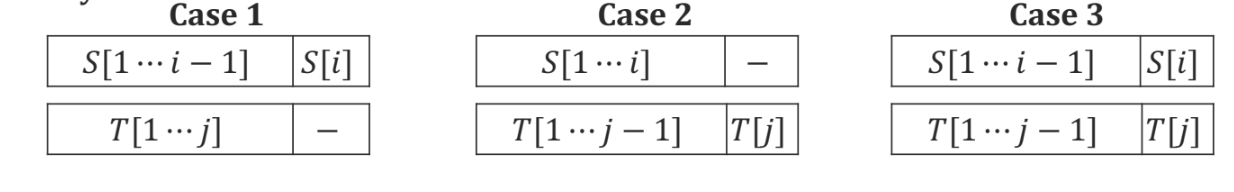
\includegraphics[scale=0.5]{alignment.png}
					\end{center}
					\comment{We add in one at a time, so there can only be one dangling letter (or none) 
					at a time!} 
			\end{itemize}
		\item We recurse based on the cases:
			\begin{itemize}
				\item Case 1: $S(i, j) = S(i-1, j) + 1$.
				\item Case 2: $S(i, j) = S(i, j-1) + 1$. 
				\item Case 3: $S(i, j) = S(i-1, j-1) + 1(S[i] \neq T[j])$.
				\item Base cases: $S(i, 0) = i$, $S(0, j) = j$. 

				The 1 represents an indicator function that counts the number of misaligned characters.
			\end{itemize}
		\item During the recursion step, we want to fill $S(i, j)$ with the \textit{minimum} value 
			of these three, since we want to minimize the number of edits. We will store this information 
			(memoizing) in a 2D array.
		\item We have to traverse our array either row by row, column by column, or diagonally. This is because
			we need to ensure that all three subproblems that we're considering have already been 
			computed. 
		\item Pseudocode:
			\begin{center}
				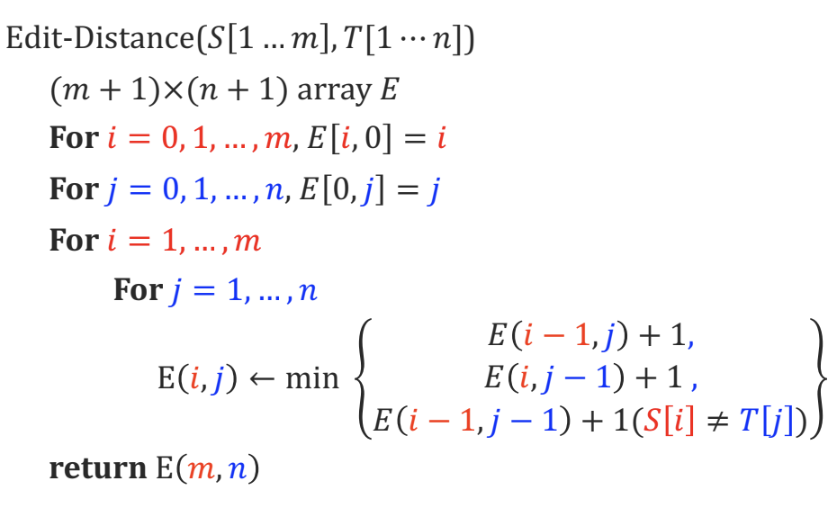
\includegraphics[scale=0.5]{alignment-pseudocode.png}
			\end{center}
		\item Runtime: there are $O(mn)$ subproblems, since we have a 2D array of dimension $mn$. At each 
			subproblem, we are only computing a minimum, which is $O(1)$ runtime, so we just have 
			$O(mn)$ runtime. 
			
			\question{Isn't the indicator also computed at this step? Why is that not accounted in the runtime?}

			\answer{The indicator is run in constant time, since we're only looking at the $i$-th character 
			in comparison to the $j$-th character.}
	\end{itemize}
	\subsection{Knapsack (with repetition)}
	\begin{itemize}
		\item A weight capacity $W$ and $n$ items with weights and values $(w_i, v_i)$. We want to output
			the most valuable collection of items whose total weight is at most $W$.
		\item We will be selecting with repetition here, but there is an easier variation where we don't
			consider repetition.
	\end{itemize}
	\subsubsection{Subproblems}
	\begin{itemize}
		\item For all $c \le W$, we want to consider the best achievable arrangement for knapsack of 
			capacity $c$. 
		\item Recurrence: For a given item $i$, then once we put it in the knapsack there are only $
			c - w_i$ capacity that remains to be optimized. This is our recurrence relation.
			\[
				K(c) = \max_{i : w_i \le c}\{v_i + K(c - w_i)\} 
			\] 
			This is a maximum over the value because we want to maximize the value being put in our 
			knapsack.
		\item We will store this information in an array of size $W + 1$, since we need a $K(0)$ element.
			\begin{center}
				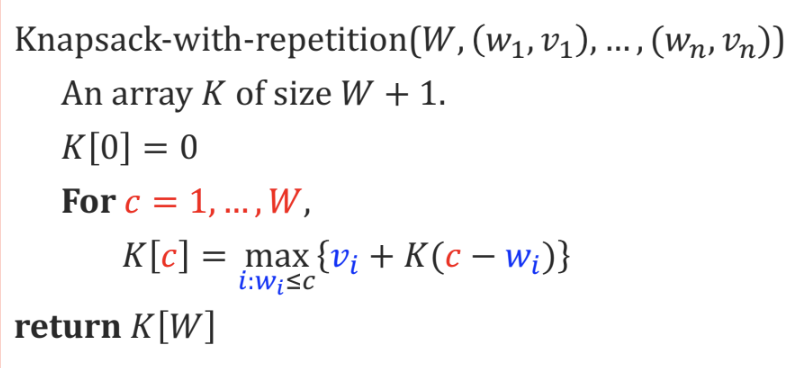
\includegraphics[scale=0.5]{knapsack-repetition.png}
			\end{center}
		\item Runtime: There are $O(W)$ subproblems, and at each subproblem, we have maximally $n$ items
			 we need to check. So in total, we have $O(nW)$ runtime.
		 \item Generally we want to think of the runtime in terms of the input. For graph problems, we looked 
			 at the input size $|V|$ and $|E|$. But for this problem, $W$ takes $\log(W)$ bits to represent 
			 $W$. So the input size is $\log(W)$. For the weights of the items themselves,
			they also only have at most $\log(W)$ bits, Therefore, the total runtime is $O(n \log W)$. 

			This kind of algorithm is polynomial in $n$, but not $W$. This is called a \underline{pseudo-
			polynomial} algorithm, since it's an algorithm that's polynomial given the numerical value 
			of the input but not in the input size.
	\end{itemize}

	\section{Dynamic Programming III}

We'll look at more examples today of DP.

\subsection{Knapsack (without repetition)}
\begin{itemize}
	\item Start with a recap with knapsack: had a weight capacity $W$, and a set of items with individual 
		weights $(w_i, v_i)$, and we wanted to look at the most valuable combination of items.
	\item Now, we're going to look at this problem with the with the constraint that \textit{we cannot 
		choose with repetition}
	\item To solve, look at how we solved the problem with repetition: introduced $K(c)$ which gets us 
		the best achieveable value for a capacity $c \le W$. The issue with trying the same thing 
		is that our subproblems don't track which items have already been used. Why not keep track of both? 
\end{itemize}

\subsubsection{Subproblems}
\begin{itemize}
	\item Introduce a 2D array: essentially solve the problem for smaller knapsacks and also smaller 
		capacities. Then expand in two directions: in terms of the number of items and also the 
		capacity.
	\item So keep track of all weights $c \le W$ and all items $j \le n$. Define $K(j, c)$ to be the 
		optimal solution to the knapsack for capacity $c$ and items $\{1, 2, \dots, j\} $. (It doesn't 
		need to use all the items from 1 to $j$.
	\item For each $K(j, c)$, we recurse smaller subproblems:

		\textit{Case 1:} The optimal solution on items 1 through $j$ doesn't use item $j$. 
					Here, $K(j, c) = K(j-1, c)$.

			\comment{Note that this is not equivalent to $K(j-1, c - w_j)$, since the $w_j$ could be 
			distributed among other items.}

		\textit{Case 2:} the optimal solution on items 1 through $j$ uses item $j$.
		Here, $K(j, c) = K(j-1, c - w_j) + v_j$. We add $v_j$ to $K$ since we're now using item $j$.   

		The intuition here is that we use the optimal solution without item $j$, then add in item $j$ 
		at the end. 
\end{itemize}
\subsubsection{Implementation}
\begin{itemize}
	\item So let's formalize this:
		\[
			K(j, c) = \max\{ K(j-1, c), v_j + K(j-1, c - w_j)\}
		.\]
		with base cases $K(0, c) = 0$ and $K(j, 0) = 0$. The base cases make sense since with no items our 
		optimal value is 0, and with no allowed weights then the optimal value is also 0. 

	\item Looking at $K(j, c)$ it only relies on the subproblmes $K(j-1, c)$, or $K(j-1, c - w_j)$, so we're 
		only looking at row $j-1$, and different elements in that row. This tells us about the order in which 
		we should be solving the subproblems: we could either do this row by row or column by column. 
	\item For runtime, ther eare $O(nW)$ subproblems, and in each subproblem we're doing constant 
		work (memory access), so therefore the total runtime is $O(nW)$, just like knapsack with repetition. 
	\item For space complexity, notice that each $K$ only depends on the previous row, so once we've 
		moved onto the 3rd row, we no longer need the first. We can delete this from memory, so the optimized 
		space complexity is $O(W)$. 
\end{itemize}
\subsection{Traveling Salesperson Problem}
\begin{itemize}
	\item A notoriously difficult problem, and DP helps us get a \textit{slightly} better runtime. 
	\item Input: Cities $1, \dots, n$ and pairwise distances $d_{ij}$ between cities $i$ and $j$. We want to 
		find a ``tour'' of minimum total distance (so we need to visit every city exactly once and 
		return to the city we started at).
	\item The naive brute-force algorithm basically is the one where we have to go through all possible 
		tours: there are \( n! \in O(n^n) \) possible tours, which makes this computation very expensive. 
	\item Dynamic programming gives us $O(n^2 2^n)$. (this is nearly optimal, beating $O(n 2^n)$ is theorized
		to be impossible)
		\begin{itemize}
			\item To give an illustration of the difference DP makes, if $n = 25$, then $O(n!) \approx 10^{25}$, 
				whereas $O(n^2 2^n) \approx 10^{10}$, so we're already better by 15 orders of magnitude. 
		\end{itemize}
\end{itemize}
\subsubsection{Subproblems}
\begin{itemize}
	\item One challenge of TSP is that subproblems aren't exactly solving the problem. If we just look at 
		TSP for a subset of our graph, that doesn't necessarily give us a solution to the larger problem, since 
		we're looking for cycles. Instead, we think of ``partial solutions'' to our graph. 
	\item We think of the subproblmes as starting from city 1, ends in city $j$, and passes thorugh all cities
		in a set $S$ (which includes city 1 and \( j \)). Visually:
		\[
			1 \to i_1 \to i_2 \to \dots \to j			
		\]
		So we want to formally define $T(S, j)$ to be the length of the shortest path visiting 
		all cities in $S$ exactly once, starting from 1 and ending at $j$. 
\end{itemize}
\subsubsection{Recurrence Relation}
\begin{itemize}
	\item How to compute $T(S, j)$ using smaller subproblems? Well, look at the string again:
		\[
			\overbrace{\underbrace{1 \to i_1 \to i_2 \to \dots \to i}_{T(S \setminus j, i)} \to j}^{T(S, j)}
		\]
		To actually talk about $T(S, j)$, then we need to add $d_{ij}$ onto every $T(S \setminus j, i)$. However,
		what is annoying is that we actually don't know which city is second to last, so we'll need 
		to consider every possible city $S \setminus j$. 
	\item So, we'll have to pick the minimum over all $i \in S$ such that $i \neq j$. Formally:
		\[
			T(S, j) = \min \{T(S \setminus j, i) + d_{ij} | i \in S \land i \neq  j\} 
		\]
	\item Our base cases are $T(\{1\} , 1) = 0$, this is fairly trivial. We also want that $T(S, 1) = \infty$.
		The reason we want this is because we're talking about incomplete paths, so $T(S, 1)$ is not 
		a valid non-cycle. Hence, we want to set it to $\infty$.  
	\item We're not done though, because we have to do something to get us back to a cycle! At the end of 
		the recursion step, we'll want to add the final edge $(j, 1)$ back, but adding only the minimum:
		\[
			T(S, 1) = \min_{j \neq  1}\{T(\{1, \dots, n\}, j) + d_{j 1}\}
		\] 
\end{itemize}
\subsubsection{Implementation}
\begin{itemize}
	\item Want an array of size $2^n \times n$, and start with base cases. Then work on the recursion:
		\begin{center}
			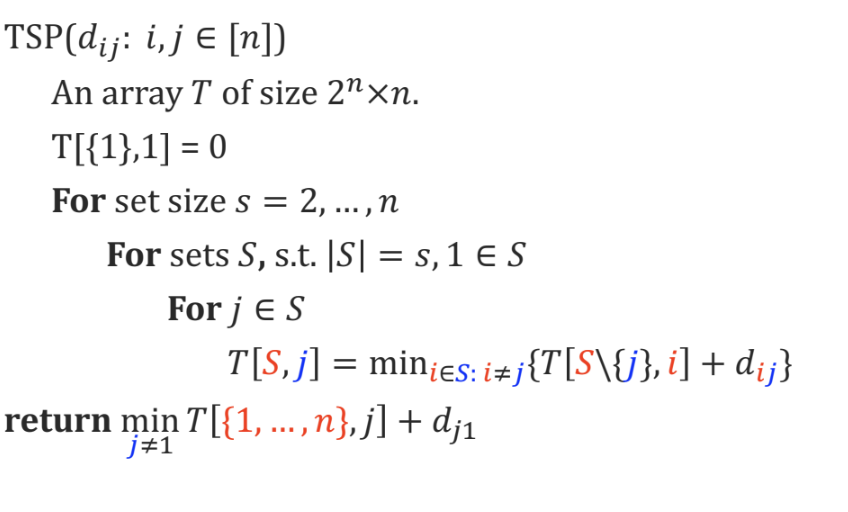
\includegraphics[scale=0.5]{TSP-code.png}
		\end{center}
	\item For runtime, there are $O(2^n \times n)$ subproblems, and on each layer we're doing $O(n)$ work, since
		we're checking the minimum across $n$ nodes every iteration. So, we have $O(n^2 2^n)$ as 
		the final runtime. 

		\question{How do we explain that \(n^2 2^n\) is the number of subproblems?}

		\answer{$O(n)$ work at every step, then $n \times 2^n$ subproblems. There are $2^n$ subsets, and in 
			each subset we can choose a $j$ to exclude, which we can upper bound by saying that there are $n$ 
		of these. So $n \times 2^n$ is a tight upper bound on the number of subproblems.}
\end{itemize}
\subsection{Independent Sets in Trees}
\begin{itemize}
	\item We're given an undirected graph \(G = (V, E)\), and want to output the largest independent 
		set of \(G\).
	\item Recall that a set \(S \subseteq V\) is considered independent if there are no 
		edges between \(u, v \in S\).
	\item This is also a notoriously hard problem, for general graphs. There isn't a polynomial time algorithm 
		that does this. But for trees, we're in luck!

		\question{Why isn't the solution just selecting every other layer?} 

		\answer{There are instances where we can pick from two consecutive layers and still not have an edge. 
		Consider the tree:
			\begin{center}
				\begin{tikzpicture}
					  \node {A}
					child {node {B}}
					child {node {C}}
					child {node {D}
					  child {node {E}}
					  child {node {F}}
					};
				\end{tikzpicture}
			\end{center}
			Our greedy algorithm would select either \(\{A, E, F\} \) or \( \{ B,C,D\} \), but the optimal set
			is actually 
		\(\{B, C, E, F\} \), so this proves that our algorithm isn't optimal.}
	\item For trees, we know that they don't have cycles, so we can pick any node and say that that is the root.
		By doing this, we can get a ``natural ordering'' of the subproblems. 
\end{itemize}

\subsubsection{Subproblems}
\begin{itemize}
	\item Let \(I(v)\) be the size of the maximum independent set in the subtree that is rooted at \(v\). 
	\item Why is this a good subproblem? Becuase it's easy to write a recursion relation for it!
	\item For the subproblems, there are two cases:

		\textit{Case 1:} \(v\) (the root of the tree) is part of the optimal independent set. This 
		means that the children aren't allowed to be part of the independent set. So if we take $v$, we can't 
		take any of the subproblems. So we need to look instead at the \textit{grandchildren} of \(v\) to join.
		Here, we'd write this as:
		\[
			I(v) = 1 + \sum_{u\  \in \text{ grandchildren}} I(u)
		\] 
		We add 1 here because we're including \(v\) now. 

		\textit{Case 2:} \( v\) is not part of the optimal independent set. Here, we would just take 
		the maximum of the children. Then:
		\[
			I(v) = \max_{u \ \in \text{ children}} \{I(u)\} 
		\] 


		So we'll take the max of these two cases:
		\[
		I(v) = \max \{1 + \sum_{u \ \in \text{ grandchildren}} I(u), \sum_{u \ \in \text{ children}} I(u)\}
		\] 
		Also, base cases is that $I(\text{leaf}) = 1$. 
\end{itemize}
\subsubsection{Implementation}
\begin{itemize}
	\item We need a data structure to store the tree easily, and also make sure that every child is processed 
		before the parents are. Well, we can iterate through the graph in post decreasing post order! 
	\item The runtime of DFS on trees is \(O(|V|)\), and each edge is looked at \(\le 2\) times -- once 
		for the children and also once for its grandchildren, so each subproblme takes constant time. 
	\item So that the total work is \(O(|E|) = O(|V|)\), since \(|E| = |V| - 1\).
\end{itemize}

	\section{Nearest Neighbor and Metric Learning}
\subsection{Parametric vs. Non-Parametric Models}
\begin{itemize}
	\item So far, we've mostly focused on parametric models, where we aim to learn \( p(y \mid x) \), through
		the use of a parameter \( \theta \):
		\[
			p_{\theta}(y \mid x) \approx p(y \mid x)
		\]
	\item The parameters are determined through MLE (or some other method), and generally the data is then
		thrown away. Today, we will look at non-parametric models (i.e. models which don't consider a
		parameter \( \theta \)). In this case, we will keep the training examples, and in effect the number
		of training parameters grows with \( n = |\mathcal{D}| \). In some sense, the dataset itself is the
		parameters. 
	\item As an aside, we should cover metric spaces first: a metric space is a set \( X \) together with a
		notion of distance \( d \) between its elements:
		\begin{enumerate}[label=\arabic*.]
			\item \( d(x, x) = 0 \).
			\item \( d(x_1, x_2) > 0 \) if \( x_1 \neq x_2 \).
			\item \( d(x_1, x_2) = d(x_2, x_1) \).
			\item Triangle inequality. 
		\end{enumerate}
		One metric we commonly see in ML is called the \textit{Mahalanobis distance}, written as:
		\[
			d_M(x_1, x_2) = \sqrt{(x_1 - x_2)^{\top} M (x_1 - x_2)}
		\]
		this collapses to the Euclidean distance when \( M = I_d \).
\end{itemize}
\subsection{KNN Classifier}
\begin{itemize}
	\item Suppose you've classified some data into two classes, and now you want to classify a new point \( x
		\). To do this, we first find the \( K \) closest (using a metric \( d \)) examples in the
		pre-existing data to inform our decision on what \( x \) should be classified as. We denote this set
		as \( N_K(x, \mathcal{D}) \). 

		\question{How is the pre-existing data generated?} 
	\item We then look at the labels \( y_i \) for the points \( N_K(x, \mathcal{D}) \), and use it to
		estimate what \( p(y \mid x)  \) should be (i.e. what label we assign it):
		\[
			p(y = c \mid x, \mathcal{D}) = \frac{1}{K}\sum_{i \in N_k(x, \mathcal{D})} I[Y_i = c]
		\]
		note that this probability sums to 1 when we sum over all \( c \), so this is actually a valid
		probability distribution. In words, this means that the probability a point \( y \) is assigned a
		label \( c \) is given by the proportion of the nearest \( K \) points that are assigned \( c \).
	\item The \( k = 1 \) case is special - the partition that you get is called a \textit{Voronoi
		tessellation}. In this case, if you scatter some points onto the plane, then this division will
		partition the space up strictly based on distance and all the boundaries are just straight edges
		between classes.  

		In this special case, the classification of a new point is given by the nearest neighbor, so this is
		why you get such a special pattern.

		\question{How do you tell the classifier how many classes you should make?} 

		\answer{This is probably something you decide ahead of time; there's probably no way for you to
		"train" a model to know how many you should make.}
	\item Visually, you can also compare different \( K \) and \( K' \) nearest neighbor algorithms, and
		there is a distinction between them. For larger \( K \), the general trend is that the boundary
		between classes gets finer and not as jagged, as is typically seen in a smaller \( K \).  
	\item There is also an optimal \( K \) for classification. If \( K \) is too large, then you risk
		comparing against points that are not near your target point \( y \), and therefore you will get a
		bad classification from it. 

		This is also a general trend we observe in model training: as the model complexity increases, the
		training error decreases monotonically, but the test error reaches an optimum somewhere in between.
		This is because there are two regimes on the extremes: extreme simplicity on one end, and overfitting
		on the other. 
\end{itemize}

\subsection{KNN Generative Classifier}
\begin{itemize}
	\item Now we move to the \( K \)-nearest neighbors except this time we have a generative classifier. In
		this case, we essentially define a "ball" around each point \( x \) until we encounter \( K \)
		points, and the classification is then given by the proportion of points in that ball \( V_K(x) \)
		that are classified as class \( c \).      
	\item If you have a \textit{lot} of data, it has been shown that the KNN test error can never be worse
		than twice the optimal Bayes classifier. This is interesting to note, because the Bayes classifier
		requires \textit{much} more information about your data (the class conditionals, distribution, etc.),
		but KNN knows nearly nothing.  
	\item This is a quick aside, but basically the idea is that the space you need to check increases
		exponentially with dimension. Because the volume grows exponentially large, it becomes increasingly
		more impractical to search such a space, and so this makes KNN much worse in higher dimensions.  

		If you want to get \( \epsilon \) close to a target, by increasing the dimension you can only get 
		\( O(n^{ - 1 / d}) \) closer to the target by increasing the dimension. 
\end{itemize}

\subsection{Pros and Cons of KNN}
\begin{itemize}
	\item Pros:
		\begin{itemize}
			\item Fast, no training required.
			\item Learns complex classification functions easily, because it requires no priors.
		\end{itemize}
	\item Cons:
		\begin{itemize}
			\item High storage cost
			\item Slow at computing inference (actually performing the classification)  
			\item Very bad dimensionality scaling. 
		\end{itemize}
\end{itemize}

\subsection{Manifold Hypothesis}
\begin{itemize}
	\item The manifold hypothesis basically states that "true" high dimensional data that we care about, like
		images, videos, etc. lie in a lower dimensional manifold which is embedded in a higher dimensional
		space.   
	\item The idea then is that we essentially "embed" the data onto a lower dimensional space using a neural
		network, learn the
		space using a Euclidean metric, then you can classify using this Euclidean metric. 

		\question{Is this the approach that t-SNE uses?}
	\item The challenge then becomes: how do you define an embedding that does exactly what you want?
		Ideally, you want an embedding that pulls similar objects close to each other and pushes dissimilar
		ones apart.
	\item One of the earliest approaches to doing this was based on \textit{contrastive loss}. Basically,
		define a loss function over two points \( i, j \):
		\[
			\mathcal{L}_{ij}(\theta; m) = \mathbb I (y_i = y_j)d(z_{\theta}(x_i), z_{\theta}(x_j))^2
			+ \mathbb I (y_i \neq y_j) \max(0, m - d(z_{\theta}(x_i), z_{\theta}(x_j))^2)
		\]
		(recall that \( z(x) \) is your embedding function). 
		Essentially, you minimize the loss between similar points, while also defining a "maximum acceptable
		distance" between two dissimilar points. You require this \( m \) because otherwise, your model will
		want to push dissimilar points increasingly farther away off to infinity.  

		Tested this on the MNIST dataset and bringing this down to a 2-dimensions from 784 dimensions, and
		the results look very good.    
	\item The problem with this approach is that the "pull" and "push" terms don't talk to each other, or in
		other words this is a very binary way to approach this embedding approach. 
	\item This leads to the second approach: triplet loss. Here, the loss is given by:
		\[
			\mathcal{L}_i(\theta; m) = \max(d(z_\theta(x_i), z_{\theta}(x_i^{+}))^2 - d(z_{\theta}(x_i),
			z_{\theta}(x_i^{-}))^2 + m, 0)
		\]
		In essence this does the exact same thing: you want the first term to decrease while simultaneously
		wanting the second term to increase, but this is a more clever approach because the terms are
		combined together. 
		
		Here, \( z^{+} \) is a positive (similar) example, and \( z^{-} \) is a dissimilar (negative)
		example.  

		\question{what is the positive and negative example referring to?} 

		\answer{these are \textit{anchors} in the data, and are given as true points in the dataset.}  
	\item One issue with the triplet loss is that because there are a lot of negative examples to compare to,
		you naturally need to perform that computation many many times to get the loss for a single point.
		This leads to the \( N \)-pair loss, which lets you take a batch of negaitve samples at a time:
		\[
			\mathcal{L}(\theta; x, x^{+}, \{x_k^{-}\}_{k = 1}^{N}) = \log\left( 1 + \sum_{k = 1}^{N -
			1}\exp\left( \hat{z}_\theta(x)^{\top} \hat{z}_\theta(x_k^{-}) - \hat{z}_\theta(x)^{\top}
			\hat{z}_\theta (x^{+}) \right) \right)
		\]
		what this means is that you take a set of predefined dissimilar examples \( \{x_k\} \) and use that
		as the "push" term. 

		\question{How does this algorithm work in practice? Would you have to define a set of similar and
		dissimilar classes for every class you're working with?} 

		\comment{The reason you don't need a max function here is because \( \hat{z}_\theta(x) \) is a
			projection that only projects into a volume of a unit sphere, so there is a predefined limit to
			how far apart dissimilar points can be apart. You can also convert this interpretation into an
		equivalent one using softmax.}   
	\item There's also the world of joint embeddings: where text and images are encoded together and embedded
		onto a space: OpenAI's CLIP model was trained on an \( N \)-pair loss in a jointly embedded space.  
\end{itemize}

	\section{Network Flow}
\begin{itemize}
	\item Recently declassified (1999) document about the USSR's shipment capacity from east to west. This 
		was crucial information at the time since had a war broke out, the US could identify which 
		supply routes they could bomb.
	\item They devised a greedy algorithm called ``flooding,'' but this algorithm wasn't really optimal. It 
		was finally solved by Ford and Fulkersson, and is now called the Ford-Fulkersson algorithm.
	\item Given a directed graph $G = (V, E)$, one source vertex $s$ and a sink $t$, and for each edge $e \in E$,
		we're given a capacity $c_e$ which are integers. 
	\item We want to find the maximum amount of water from $s \to t$.  
	\item \textit{Definition:} A flow assigns a number $f_e$ to each directed edge $e \in E$ such that:
		\begin{itemize}
			\item nonnegativity: \(f_e \ge  0\) 
			\item capacity: \(f_e \le c_e\)
			\item flow in and flow out are equal: \(\sum_{u \to v} f_{u, v} = \sum_{v \to w} f_{v, w} \)
		\end{itemize}
	\item Let's also define the size of the flow $f$ to be the total quantity set from $s$ to $t$. Using 
		this definition, then the maximum flow is the one that maximizes $\size(f)$. This can be solved 
		using linear programming!
\end{itemize}

\subsection{Greedy (suboptimal) algorithm}
\begin{itemize}
	\item We'll find a path $P$ from $s$ to $t$, and send flow until it's saturated. We'll do 
		this as much as we can. We repeat this until we run out of paths.
	\item This algorithm fails on some graphs, because it uses edge $A \to B$ when that edge is suboptimal! 
		Consider the graph:
		\begin{center}
			\begin{tikzpicture}[scale=2]
				\node (s) at (0, 0) {$s$};
				\node (a) at (1, 0.7) {$A$};
				\node (b) at (1, -0.7) {$B$};
				\node (t) at (2, 0) {$t$};
				\graph[edge label = 1]{(s) ->(a) -> (t), (s) -> (b) -> (t), (a) -> (b)};
			\end{tikzpicture}
		\end{center}
		Our algorithm just looks at flow rate, so a possible path to take is $s \to A \to B \to t$, but this 
		is clearly suboptimal! Instead, we should be going from $s \to A \to t$ and $s \to B \to t$. 
\end{itemize}

\subsection{Greedy Fix}
\begin{itemize}
	\item We instead consider a residual graph, where we subtract the flow given by greedy 
		($s \to A \to B \to t$), and also generate a back edge that travels in the reverse order of the flow 
		given by greedy, so that we can backtrack if needed. 
	\item Formally, given a graph $G$ and a flow $f$ on $G$, the residual raph $G_f$ is defined as:
		For all edges \((u, v)\), if $f$ goes from $u \to v$, then the residual graph will flow from $v \to u$ 
		and the edge will have capacity $c_{u, v} - f_{u, v}$. 

		By doing this, we allow our graph to backtrack along our suboptimal path if needed.  
	\item This is the approach that Ford Fulkerson uses to find the optimal flow.
\end{itemize}

\subsection{Ford-Fulkerson Algorithm}
\begin{itemize}
	\item Find a path $P$ from $s$ to $t$ in the residual graph which is not yet saturated, and send more 
		flow along $P$. We keep repeating this until everything's saturated, and this happens 
		when all edges along one particular cut is zero. 
	\item To show that this algorithm terminates, lets' first define an $s-t$ cut is a partition of the graph
		into two sets of vertices \(L\) and \( R\) such that 
		\(s \in L\) and \(t \in R\). We define the capacity of this cut to be the sum of all capacities from 
		the edges that cross from $L$ to $R$.  
	\item Therefore, for any flow $f$ and any cut \((L, R)\), then \(\size(f) \le \capacity(L, R)\). Then, the
		flow is actually upper bounded by the minimum cut along this graph (this is our ``bottleneck'' introduced
		at the outset)
	\item Then, this means that the max flow is also given by the minimum cut, and we can show that 
		Ford-Fulkerson outputs a maximum flow by considering this relation between the flow and a cut. The proof 
		of this is outlined in lecture. 

		\question{Review the proof for this later}
\end{itemize}

\subsection{Runtime}
\begin{itemize}
	\item The number of augmenting paths must be less than $U$, where $U$ denotes the maximum flow, so 
		the update is less than $O(m + n) \cdot U$. 
	\item But what this means   
	\item There are other algorithms out there that optimizes this a little more: Edmonds-Karp gives 
		us a runtime of $O(n m^2)$, which is much better than what we have. 
	\item The best runtime was discovered last year, where we have $O(m^{1 + o(1)} \cdot \log U)$
\end{itemize}

	\section{Laplace Transform}
\begin{itemize}
	\item Laplace transforms concern the equation:
		\[:tabn
		X(s) = \int_{-\infty}^{\infty} x(t) e^{-st} \diff t
		\] 
		The basic idea is that instead of solving for \( x(t) \), we solve instead for \( X(s) \), which is 
		much easier to do sometimes than \( x(t) \). 
	\item Suppose you have an LTI system with impulse response \( h(t) \), and we input a harmonic 
		exponential \( e^{j 2\pi ft} \), then we get an output \( y(t) = H(f) e^{j 2 \pi ft}
		= H(\omega) e^{j \omega t}\). (this is the 
		eigenfunction property.)
	\item What about an input \( e^{st} \)? Then, we can express this as a convolution, which 
		happens to be written as: \( y(t) = H(s) e^{st} \), where  \( H(s) \) is the Laplace transform of 
		\( h(t) \). 
	\item Consider an input \( x(t) = e^{st} \), and since \( s \in \C \), then we can write 
		\( s = \sigma + j \omega \). Then we convolve:
		\[
		y(t) = \int_{-\infty}^{\infty} h(t) e^{s(t - \tau)}\diff \tau = \int_{-\infty}^{\infty} 
		h(t) e^{st} e^{-s \tau}\diff \tau = e^{st}\underbrace{\int_{-\infty}^{\infty} h(\tau) e^{-s \tau}\diff \tau}
		_{H(s)}
		\] 
		where the integral we defined earlier as the Laplace transform \( H(s) \). Here, we call it 
		specifically the bilateral Laplace transform of \( h(t) \). This distinction just has to do with the 
		integration bounds; a unilateral Laplace transform is defined as 
		\[
		H_{\text{uni}}(s) = \int_{0}^{\infty} h(\tau)e^{-s \tau}\diff \tau 
		\] 
		but we will normally consider bilateral Laplace transforms in this class.  
	\item Note also that the Laplace transform is also the more general case of the Fourier transform: the Fourier
		transform occurs when \( \Re(s) = 0 \). 
\end{itemize}
\subsection{Notation, Terms}
\begin{itemize}
	\item With Laplace transforms, we say that they transform between the time domain and the \( s \)-domain, and 
		it's written as:
		\[
		\mathcal L \{x(t)\}  = X(s) = \int_{-\infty}^{\infty} x(t) e^{-st}\diff t 
		\] 
		Because \( s \) is a complex number, the Laplace transform takes our 1-dimensional signal 
		\( x(t) \) and turns it into a two-dimensional signal in  \( s\)-space. 
%		\begin{center}
%			\begin{tikzpicture}
%				\draw (-3, 0) -- node[right] {\( t \) } (3, 0);
%			\end{tikzpicture}
%			\( \rightarrow \) 
%			\begin{tikzpicture}
%				\draw(-3, 0) -- (3, 0) node[right] {Real};
%				\draw (0, -3) -- (0, 3) node[left] {Imaginary};
%				\draw[red] (0, 0) -- node[right] {\( X(s) \) } (1, 2);
%			\end{tikzpicture}
%		\end{center}
\end{itemize}
\subsection{Laplace Transform Pairs}
\begin{itemize}
	\item Given a signal \( x(t) = \delta(t) \), then the Laplace transform \( X(s) = 1 \). This is seen easily 
		from the integral itself:
		\[
		X(s) = \int_{-\infty}^{\infty} \delta(t) e^{- st}\diff t = 1 
		\] 
		As a 2D diagram, we can imagine that over the entire complex plane, \( X(s) \) takes on a value 
		of 1. 
	\item Given a unit step function \( x(t) = u(t) \), then the Laplace transform \( X(s) = \frac{1}{s} \). 
		Again, just do the integral:
		\[
		X(s) = \int_{-\infty}^{\infty} u(t) e^{-st}\diff t = \int_{0}^{\infty} e^{-st}\diff t = \frac{1}{s} 
		\] 
		Note that this only works if \( \Re(s) > 0 \), otherwise we have an unbounded integral. This condition 
		is also called the \textit{region of convergence} for the integral. This actually means that 
		the Laplace transform may not be defined for all values of \( s \)!

		\comment{Note that \( \Im(s) \) doesn't matter here, since all it does is give us an overall phase 
		factor of \( e^{j \omega t} \) that has magnitude 1 all the time.}
	\item Let \( x(t) = e^{-at}u(t) \). Then, let's look at its Laplace transform:
		\[
		X(s) = \int_{-\infty}^{\infty} e^{-at}u(t) e^{-st}\diff t = 
		\int_{0}^{\infty} e^{-(a + s)t}\diff t  = \frac{1}{a + s}
		\] 
		which again, only holds true when \( \Re(a +s) > 0 \). Since \( a \) is real, then the condition 
		simplifies to \( \Re(s) > -a \), so this is our region of convergence.  
		
		\comment{We could be a little more specific with the integration:
			\[
			X(s) = \int_{0}^{\infty} e^{-(a + \sigma)t} e^{- j \omega t} \diff t = \frac{1}{j \omega ( + a + \sigma)}
			 = \frac{1}{s + a}
			\] 
			but this simplifies in the same way.  
		}

		\question{If we didn't have the \( u(t) \), then would the integral still converge?}
	\item Now consider \( x(t) = -e^{-at}u(-t) \). This is just the time-flipped version of the previous signal. 
		Visually, for different values of \( a \), this is what it looks like:
		\begin{center}
			\begin{tikzpicture}[scale=0.2]
				\draw (-10, 0) -- (10, 0);
				\draw (0, -10) -- (0, 10);
				\draw[thick, color=red, domain=0:-2]  plot (\x, {-exp(-\x)}) node[left] {\( a > 0 \) };
				\draw[thick, color=blue, domain=0:-8] plot (\x, {-exp(\x)}) node[above left] {\( a < 0 \) };
			\end{tikzpicture}
		\end{center}
		Doing the Laplace transform:
		\[
		X(s) = -\int_{-\infty}^{\infty} e^{-at}u(-t)e^{-st}\diff t  = \int_{-\infty}^{0} e^{-(a + s)t}\diff t
		= \frac{1}{a + s}
		\] 
		As before, this only holds when \( \Re(a + s) > 0 \). 

		\question{Mathematica gives \( -\frac{1}{a + s} \), why?}
\end{itemize}
\subsection{Why Laplace Transform?}
\begin{itemize}
	\item Laplace transform has many of the same properties as the Fourier transform, and due to its 
		wider scaope (i.e. having \( X(s) \) be a two-dimensional function), it allows us to take the transform of 
		functions that the Fourier transform cannot handle. 
	\item It's also useful for integral differential equations. Consider the following circuit:
		% tikz here
		The voltage readout is given by:
		\[
		Ri(t) + \left[ \frac{1}{\mathcal L }\int_{0^{-}}^{t} i(t') \diff t' + v_c(0^{-})  \right] 
		\] 
		we will see later on how the Laplace transform simplifies the calculation of this integral.  
\end{itemize}

\subsection{Region of Convergence}
\begin{itemize}
	\item The Laplace transform is also related to the Fourier transform, by a multiplication of a 
		decaying exponential:
		\[
		\mathcal L \{x(t)\}  = \mathcal F \{x(t) e^{-\sigma t}\} 
		\] 
		This also tells us why the Laplace transform is more general -- by multiplying by an 
		\( e^{-\sigma t} \), we can actually modify what \( x(t) \) is. This gives us more control, and makes 
		it a more powerful tool. 
		
		The region of convergence is defined as the set of \( s \in \C \) suhc that 
		\( x(t) e^{-st} \) has a Fourier transform. Mathematically:
		\[
		\mathcal L \{x(t) \}  = \int_{-\infty}^{\infty} x(t) e^{-at} e^{- j \omega t}\diff t  < \infty
		\] 
		We've already talked a lot about the region of convergence in the previous section, so just refer to that 
		instead. 
	\item Consider the signal \( x(t) = 3d^{-2t}u(t) - 2e^{-t}u(t) \). What is its region of convergence? Since the 
		Laplace transform is linear, we can basically just find the region of convergence for both these 
		terms, and find the common ROC to get the ROC for \( X(s) \). Doing so, we get:
		\[
		X(s) = \frac{3}{s + 2} - \frac{2}{s + 1} = \frac{s - 1}{(s + 2)(s + 1)}
		\] 
		Therefore, the region of convergence is \( \Re(s) > -1 \). 
\end{itemize}

\subsection{Properties of Laplace Transform}
\begin{itemize}
	\item These are very similar to the Fourier transform properties. We will denote the relationships 
		as \( x(t) \overset{\mathcal L}{\leftrightarrow} X(s) \). 
	\item \textbf{Linearity:} Given  \( ax_1(t) + bx_2(t) \), then the Laplace transform gives \( aX_1(s) + bX_2(s) \).
		The region of convergence contains \( R_1 \cap R_2 \), but it can be larger. For example, if you take 
		a signal with some limited ROC and consider  \( x_1(t) - x_1(t) \), then the ROC would now turn into the 
		entire plane!
	\item \textbf{Time shift:} Given \( x(t - t_0) \), then we have \( e^{-st_0}X(s) \). Very similar to 
		the Fourier transform! The proof is relatively easy, just do a change of variables. 
	\item \textbf{S-domain shift:} Given \( e^{s_0 t} x(t) \), then this gives  \( X(s - s_0) \). Again, just 
		do the integral via a change of variables. The ROC will be shifted by \( \Re(s_0) \). 

		More formally, if we let \( s' = s - s_0 \) and it has a ROC of \( R \), then the ROC of \( s \) is 
		going to be \( R + \Re(s_0) \). 
	\item \textbf{Time scaling:} For a signal \( x(at) \), then the Laplace transform gives  \( \frac{1}{a}X(s) \).
		So if we shrink in time domain, then we expand in the \( s \)-domain, just like the Fourier transform.
		The new ROC is now \( a \cdot R \). As for the proof:
		\begin{align*}
			\int_{-\infty}^{\infty} x(at) e^{-st} \diff t  &=  \int_{-\infty}^{\infty} x(\tau) 
			e^{-s \tau / a} \frac{1}{a} \diff \tau \\
			&= \frac{1}{|a|}\int_{-\infty}^{\infty} x(\tau) e^{-s \tau / a} \diff \tau = \frac{1}{|a|}
			X\left( \frac{s}{a} \right) 
		\end{align*}
		\question{study this proof later.}
		
		There is also the case where \( a = -1 \), in which case we have \( x(-t) \overset{\mathcal L}
		{\leftrightarrow} X(-s)\). 
	\item Given a signal \( \cos(\omega_0 t) u(t) \), then we get \( X(s) = \frac{s}{s^2 + \omega_0^2} \). The strategy
		is basically the same thing as the Fourier transform, where we split the cosine into 
		complex exponential form. The region of convergence is \( \Re(s) > 0 \).

		For \( \cos(- \omega_0 t) u(-t) \), then we have \( X(s) = -\frac{s}{s^2 + \omega_0^2} \). 

		\question{check this.}
	\item \textbf{Conjugation:} Suppose we have \( x(t) \) and take the complex conjugate \( x^{*}(t) \), 
		then just like the Fourier transform where \( x^{*}(t) \) corresponds to \( X^{*}(-\omega) \), here 
		we it gives us \( X^{*}(s^{*}) \).  

		This doesn't change the ROC, since the ROC only depends on the real component. 

		\question{Isn't this different from the Fourier property, where the input is not conjugated?} 

		\answer{Because the Fourier transform deals with a purely imaginary \( s \), then swapping to a negative 
		is the same as conjugating a general complex value \( s \in \C \).}
	\item \textbf{Convolution Theorem:} We have \( x_1(t) * x_2(t)  \) transforms as \( X_1(s) X_2(s) \). The region
		of convergence here is \( R_1 \cap R_2 \), since we need a place where the Laplace transform 
		always exists. 

		The mathematical steps to prove this are nearly identitcal to what we had for the Fourier transform.
	\item \textbf{Differentiation:} The derivative \( \dv{x(t)}{t} \) transforms as \( s X(s) \). This makes 
		solving differential equations to be much more approachable. The ROC will contain \( R \), but 
		can sometimes include more than just \( R \). An example where \( R \) increases 
		is the signal \( x(t) = \sin(\omega_0 t) u(t) \). 

		We know that \( x(t) \) transforms to \( X(s) = \frac{\omega_0}{s^2 + \omega_0^2} \), then 
		\( \dv{x(t)}{t}  \) will transform as \( \frac{\omega_0s}{s^2 + \omega_0^2} \). 
	\item \textbf{Differentiation in s-domain:} The function \( -t x(t) \) transforms as 
		\( \dv{X(s)}{s} \), and the region of convergence does not change. In general, for a 
		signal \( t^n e^{-at} u(t)\), this will transform as 
		\[
		X(s) = \frac{(-1)^{n} n!}{(s + a)^{n}}
		\] 
\end{itemize}






	\section{Zero Sum Games}
\subsection{Game 1}
\begin{itemize}
	\item We saw last time that given a ZSG structured like this:
		\begin{center}
			\begin{tabular}{c|c|c}
				& P1& P2\\
				\hline 
				P1 & 3 & -1\\
				\hline
				P2 & -2 & 1
			\end{tabular}
		\end{center}
		then we can calculate that the payoff for column 1 is \(3p_1 - 2p_2\), and the payoff for column 
		2 is \(-p_1 + p_2\).
	\item This meant that the column player's best strategy was to look at these two values, and minimize this.  
	\item The row player will then pick \(p_1, p_2\) in order to maximize what the column player tries to 
		minimize. Therefore, the row player wants to calculate:
		\[
			\max_{\text{mixed strategies \(p\)}} \{\min \{3p_1 - 2p_2, -p_1 + p_2\} \} 
		\] 
	\item As we said last lecture, this can be solved using LP! We'll also see that the row player going 
		first doesn't hurt them. 
	\item So we can formulate our LP as follows:

		Maximize a quantity \(z\), subject to the constraints:
		\begin{align*}
			z & \le 3p_1 - 2p_2\\
			z &\le -p_1 + p_2\\
			1 &= p_1 + p_2\\
			0 &\le p_1, p_2
		\end{align*}
		Note that \(z = \min \{3p_1 - 2p_2, -p_1 + p_2\} \), so by maximizing \(z\) subject to these two 
		constraints means that \(z\) is constrained to the smaller of these two. 
\end{itemize}
\subsection{Game 2}
\begin{itemize}
	\item The exact same game board, except we allow the column player to go first and the row player goes 
		second. 
		\begin{center}
			\begin{tabular}{c|c|c}
				& P1& P2\\
				\hline 
				P1 & 3 & -1\\
				\hline
				P2 & -2 & 1
			\end{tabular}
		\end{center}
	\item We do the exact same thing, by considering the possibilities from the row player's perspective. This
		is the same as looking from the column player's perspective in the previous problem. 
		\begin{itemize} 
			\item From the row player's perspective, payoff of row 1 is \(3q_1 - q_2\), and row 2 is: 
				\(q_2 - 2q_1\). So we want to choose the max of these two, i.e.:
				\[
				\max \{3q_1 - q_2, -2q_1 + q_2\} 
				\] 
			\item The column player will try to minimize this score, so they'll want to choose:
				\[
					\min_{\text{mixed strategies \( q\)}} \{ \max \{3q_1 - q_2, -2q_1 + q_2\} \} 
				\] 
		\end{itemize}
	\item This is another linear program! Here, we want to minimize \(z\), subject to:
		\begin{align*}
			3a_1 - a_2 &\le  z\\
			-2q_1 + q_2 &\le z\\
			q_1 + q_2 &=  1 \\
			q_1, q_2 &\ge 0
		\end{align*}
		Again, note that \(z\) is equal to the larger of the two inequalities, using the same logic as 
		before.
	\item Now we compare the two problems, and compare the final quantities that we wanted to compute. 
		\begin{itemize}
			\item In game 1, we wanted to find \(\max_p \{\min_q \{S(p, q)\} \} \) 
			\item In game 2, we wanted to find \(\min_q \{\max_p \{S(p, q)\} \} \)
		\end{itemize}
	\item Given this construction, we have the inequality
		\[
		\max_p \{\min_q \{S(p, q)\} \} \le \min_q \{\max_p \{S(p, q)\} \} 
		\] 
		
		\question{If the dual of the dual is the original, doesn't this mean that we get a situation like 
		\(x \le  y \le  x\)?}

		\answer{No, becuase the inequality flips again, so we get \( x \le y \ge  x \), a valid inequality.}     

		The best way to see that this is true is that it's always better to be the player that 
		goes second. Therefore, finding the minimum over \(q\) is better because they're able to ``react'' to 
		the column player's moves.
	\item It turns out that these two LPs are actually duals of each other (the proof is to construct 
		the second LP from the first one). Now, recall the property of strong duality, which holds for any LP
		that is bounded. This game is clearly bounded, so we know that there is an optimal value of the game 
		(denoted by $\mathrm{Value}(\text{game})$) is the same for both games!  

		This is called the \textbf{min-max theorem.}
	\item This tells us that the order of play doesn't change the value of the game, and there is an optimal 
		probability distribution that the row player can choose without caring about what the column player 
		does. 
		
		\comment{Note that this is a zero sum game not by the game table, but because the gain of one player 
		is an equal loss in the other player. So the numbers in the table can be anything!} 
	\item This also says that all zero sum games are strongly dual.
\end{itemize}
\subsection{P vs. NP}
\begin{itemize}
	\item So far, we've seen a lot of algorithms: polynomial multiplication, MSTs, APSP, etc.
	\item In theoretical CS, we consider all these problems to be ``efficiently solvable,'' We define 
		this to be the case when a problem can be solved in \textbf{polynomial time.}

		\comment{This is only in theoretical CS. In practice, we'd want to get everything down to 
		\(O(n)\) time, if possible. Even \(O(n^2)\) is quite bad, since given an input of size 
		\(10^9\) (as is the case with the facebook graph), then the computation is on the 
		order of \(10^{18}\) (very bad)!}
	\item We define P (stands for polynomial) to be a set of computational problems that are considered to be
		efficiently solvable.  
	\item We define NP (stands for non-polynomial) to be another complexity class that aren't 
		efficiently solvable themselves, but whose 
		solutions can be efficiently checked. 
		\begin{itemize}
			\item Example: 3-coloring problem. We want to find a 3-coloring on this graph. Naively, 
				we can brute-force and try all possible combinations, which would correspond to checking 
				\(3^{n}\) possible graphs. 
			\item The best known algorithm for this solves the problem in \(1.3289^{n}\) time.  
			\item So this algorithm is not in P, but it is in NP, since any solution can be verified in 
				polynomial time (by checking all edges)
			\item Example 2: Factorization. Given an \(n\)-bit integer \(N\), we want to factorize it into 
				two numbers \(p, q >1\) such that $pq = N$. 
			\item Naively, we can divide \(N\) by every number from \(1\) to \(\sqrt{N} \). In terms of 
				time complexity, this is \(O(\sqrt{N} )\), which we can simplify this to \(O(2^{n /2}\) due to 
				the way numbers are represented as bitstrings. 

				The best algorithm runs in time \(C^{n^{1/3}} \log(n)^{2/3}\), so this is not a problem 
				that's known to be in P. 

				However, the problme is in NP, because we can just verify any solution by multiplying them 
				together, which takes at most \(O(n^2)\) time. 
		\end{itemize}
\end{itemize}

	\section{Transfer Function of LTI Systems}
\begin{itemize}
	\item For an LTI system with the standard input and output pairs, we know that since \( y(t) = x(t) * h(t) \), 
		then this means that 
		\[
		Y(s) = X(s) H(s)
		\] 
		where \( H(s) \) denotes the Laplace transform of the impulse response, 
		\[
		H(s) = \int_{-\infty}^{\infty} h(t) e^{-st}\diff t 
		\] 
	\item For an LCCDE of the form:
		\[
			\sum_{k=0}^{N} a_k \dv[k]{y(t)}{t} = \sum_{k=0}^{M} b_k \dv[k]{x(t)}{t}
		\] 
		then we can take the Laplace transform of both sides, 
		\[
		\sum_{k=0}^{N} a_k s^{k}Y(s) = \sum_{k=0}^{M} b_k s^{k}X(s)
		\] 
		So, this means that:
		\[
		H(s) = \frac{Y(S)}{X(s)} = \frac{\sum_{k=0}^{\infty} b_k s^{k}}{\sum_{k=0}^{N} a_k s^{k}}
		\] 
\end{itemize}
\subsection{RLC Circuit}
\begin{itemize}
	\item Consider the following circuit:
		\begin{center}
			\begin{circuitikz}[american]
				\draw (0, 3) to [voltage source, l_ = \( x(t) \)] (0, 0);
				\draw (0, 3) to [R] (2, 3) to [R] (4, 3);
			\end{circuitikz}
		\end{center}
\end{itemize}
\subsection{Effect of Poles}
\begin{itemize}
	\item For non-repeated poles (as in, the poles aren't degenerate), then the transfer function can 
		be written generically as:
		\[
		H(s) = \sum_{i=1}^{N} \frac{A_i}{s - a_i}
		\] 
		If the system is causal, then recall that for an LTI system this means that \( h(t) = 0 \) for \( t < 0 \)
		\[
		h(t) = \sum_{i=1}^{N} A_i e^{-a_i t}u(t)
		\] 
	\item If \( \alpha_i \) is repeated \( m \) times, then the system response will include these terms:
		\[
			t^{m-1}e^{\alpha_i t}, \cdots,te^{\alpha_1}t, e^{\alpha_i t}
		\] 
\end{itemize}
\subsection{Stability of Causal System}
\begin{itemize}
	\item Given a causal system described by  \( H(s) \), we saw earlier that \( Y(s) = H(s) X(s) \). There's also 
		a theorem that says that the system is stable if and only if all poles of \( H(s) \)  have strictly negative 
		real parts. 
		This is because of two reasons:
		
		\begin{enumerate}[label=\arabic*.]
			\item This is because if \( H(s) \) is rational, 
				then the causality is equivalent to the region of convergence to 
				the right of the rightmost pole (on the real line)
			\item The absolute integrability condition \( \int_{-\infty}^{\infty} |h(t)|\diff t < \infty \) means 
				that the imaginary axis is within the ROC. 
		\end{enumerate}
\end{itemize}
\subsection{Connected LTI Sytems}
\begin{itemize}
	\item For systems connected in series, then \( H(s) = H_1(s)H_2(s) \), and in parallel then
		\( H(s) = H_1(s) + H_2(s) \). This is the exact same as the Fourier transform \( H(\omega) \) properties. 
	\item For feedback control systems (e.g. a compensator), then we define an error function 
		\( E(s) = X(s) - H_2(s) Y(s) \). The subtraction comes from the fact that the feedback is fed 
		as a minus sign. Then, \( Y(s) = H_1(s) E(s) \), and solving both equations 
		gives:
		\[
		Y(s) = H_1(s) X(s) - H_1(s) H_2(s) Y(s) \implies H(s) = \frac{Y(s)}{X(s)} = \frac{H_1(s)}{1 + H_1(s)H_2(s)}
		\] 
\end{itemize}
\subsection{Z-transform}
\begin{itemize}
	\item Very much the same as the Laplace transform, but for discrete-time signals. 
	\item This is very similar to the DTFT formula:
		\[
			X(e^{j \omega}) = \sum_{n=-\infty}^{\infty} x[n] e^{-j \omega n}
		\] 
		This is periodic because the signal is discrete in time. The z-transform is the generalized version of this 
		formula, written as:
		\[
			X(z) = \sum_{n=-\infty}^{\infty} x[n] z^{-n}, z \in \C
		\] 
		so really, the only difference is that we swapped \( e^{-j \omega} \) for a general complex 
		number \( z \). Because \( z \) also has a magnitude term, there's also a corresponding region of 
		convergence for \( z \). 
\end{itemize}
\subsection{Pairs}
\begin{itemize}
	\item Given \( x[n] = \delta[n] \), then:
		\[
			X(z) = \sum_{n=-\infty}^{\infty} \delta[n] z^{-n} = 1
		\] 
		as long as \( z \neq 0 \). With that caveat in mind, the ROC is the entire complex plane. 
	\item Given \( x[n] = a^{n}u[n] \):
		\[
			X(z) = \sum_{n=-\infty}^{\infty} a^{n}u[n] z^{-n} = \sum_{n=0}^{\infty} a^{n}z^{-n}
			= \sum_{n=0}^{\infty} (az^{-1})^{n} = \frac{1}{1 - (az^{-1})}
		\] 
		the last step simplifies due to geometric series. The condition for this to converge is 
		that \( |az^{-1}| < 1 \), since that's when the geometric series converges. So this simplifies 
		to \( |z| > |a| \), or \( |z| > a \) since \( a \) is real. 

		Visually, this corresponds to a boundary at infinity and one that's a circle at radius \( a \). Consequently, 
		if the unit circle exists within the region of convergence, then we know that the DTFT of the signal 
		exists. 
	\item Given \( x[n] = -a^{n}u[-n - 1] \):
		\[
			X(z) = \sum_{n=-\infty}^{\infty} -a^{n}u[-n - 1] z^{-n} = \sum_{n=-\infty}^{-1} -a^{n}z^{-n}
			= 1 - \sum_{n=0}^{\infty} (-a^{-1}z)^{n}  = 1 - \frac{1}{1 - a^{-1}z}
		\] 
		The region of convergence is defined similarly: \( |za^{-1}| < 1 \), so \( |z| < |a| \). This is just a
		filled circle up to a radius of \( |a| \). Of course, the DTFT exists only when the radius of this circle 
		is larger than 1. 
	\item Given  \( x[n] = -\left( \frac{1}{2} \right)^{n}u[-n - 1] + \left( -\frac{1}{3} \right)^{n}u[n] \), 
		since the z-transform is linear, then:
		\[
		X(z) = \frac{1}{1 - 2z } + \frac{1}{1 + z^{-1} / 3} = \cdots = \frac{6z^2 - 6z - 1}{(3z + 1)(2z - 1)}
		\] 
\end{itemize}
\subsection{Z-transform properties}
\begin{itemize}
	\item The ROC for z-transforms are circles or rings instead of planes, and that's just becuase we're 
		converting \( e^{j \omega} \) to \( z \). 
	\item See the lecture slides for a table on the properties. 
\end{itemize}
\subsection{Inverse Z-transform}
\begin{itemize}
	\item We can compute the inverse Z-transform using partial fraction expansion. The reason we keep going back 
		to this is because many Z-transforms are characterized by rational functions, so if we can find a way to 
		split the fractions up then we can find the inverse from linearity.  
\end{itemize}





	\section{Reductions II}
\begin{itemize}
	\item Recap: Two computational problems \(A\) and \(B\), and \(A\) reduces (in polynomial time) to \(B\) 
		is written as \(A \preceq_p B\). This means that if an algorithm exists to solve \(B\) in polynomial 
		time, then that same algorithm can be used to solve \(A \) in polynomial time. 

		\question{Is this restricted to only polynomial time? Shouldn't any feasible algorithm that solves 
		\(B\) also solve \(A\)?}
		
		\question{Why are we so concerned about polynomial time? Do similar problems exist if we define 
		``efficient'' to be exponential time?}
	\item Also recall the diagram we made to represent this process of reducing \(A\) to \(B\), via 
		a polynomial time reduction and recovery algorithm. Note that these two algorithms \textbf{must} execute
		in polynomial time. 
		\begin{itemize}
			\item We can prove that \(A \preceq_p B\) even if \(A, B\) are not known to be efficient.
		\end{itemize}
	\item We also saw two reductions: zero sum games reducing to LP, and Hamiltonian cycle reducing to min-TSP.
	\item Transitivity: If \(A \preceq_p B \preceq_p C\), then \(A \preceq_p C\). 
\end{itemize}
\subsection{Common mistakes in Reductions}
\begin{itemize}
	\item If we're asked to prove that \(A \preceq_p B\), we need to come up with an algorithm that takes
		\(A\) to \(B\), not \(B\) to \(A\). Make sure you check that you're proving the correct direction!
\end{itemize}
\subsection{Landscape of Problems}
\begin{itemize}
	\item We're going to use the below diagram to show the problems:
		\begin{center}
			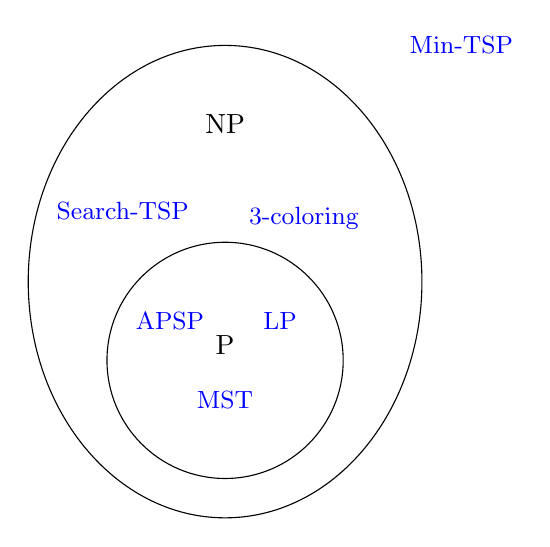
\begin{tikzpicture}
				\draw(0, 0) circle [radius=1.5cm];
				\draw node at (0, 0.2) {P};
				\draw (0, 1) ellipse [x radius = 2.5, y radius = 3];
				\draw node at (0, 3) {NP};
				\draw[blue] node at (0, -0.5) {\small MST};
				\draw[blue] node at (0.7, 0.5) {\small LP};
				\draw[blue] node at (-0.7, 0.5) {\small APSP};
				\draw[blue] node at (1, 1.8) {\small 3-coloring}; 
				\draw[blue] node at (-1.3, 1.9) {\small Search-TSP};
				\draw[blue] node at (3, 4) {\small Min-TSP};
			\end{tikzpicture}
		\end{center}
	\item We're not going to prove this, but it has been shown that factoring reduces to the 3-coloring 
		problem. Similarly, factoring also reduces to the Rudrata Cycle problem. 
	\item It turns out that every problem in NP reduces to Rudrata cycle!
	\item These are the most difficult problems in NP, and it can be shown that every problem in NP reduces 
		to an NP-complete problem
	\item \textbf{NP-Hardness:} A problem \(A\) is NP-hard if every problem \(B\) in NP reduces to \(A\). 
	\item \textbf{NP-Completeness:} A problelm \(A\) is NP-complete if \(A \in \text{NP}\) and \(A\) is 
		NP-hard.
	\item Problems in NP that aren't NP-complete are called an \textbf{NP-intermediate} problem 
	\item \textbf{Fact:} Given two problems that are NP-complete, then \(A \preceq_p B\) and \(B \preceq_p A\). 
		So this means that you can basically think of \(A\) and \(B\) are basically equivalent problems. 

		\question{Is this a biconditional?}

		\answer{No, consider two problems in P: they can be reduced to one another, but they are not 
		in NP.} 
		\begin{itemize}
			\item  There are thousands upon thousands of NP-complete problems, and by notion of reduction, 
				they are (in some sense) the same problem.
			\item This also means that if there exists a polynomial time algorithm for any NP-problem, 
				then this would imply that P = NP.
		\end{itemize}
		\question{How is it that if P = NP then every problem becomes NP-complete?}  
\end{itemize}

\subsection{Proving NP-Completeness}
\begin{itemize}
	\item Cook-Levin Theorem: showed that every problem in NP reduces in polynomial time to a circuit SAT 
		problem.
	\item It can then be shown that circuit-SAT reduces to 3-SAT, making 3-SAT an NP-complete problem. In 
		terms of a diagram:
		\begin{center}
			\begin{tikzpicture}[every text node part/.style={align=center}]
				\foreach \x in {0, 4}
						\draw[-stealth] (\x+0.5, 0) -- (\x+2, 0);
				\draw node at (-1, 0) {Every problem \\ in NP};
				\draw node at (3.25, 0) {Circuit\\SAT};
				\draw node at (7.25, 0) {3-SAT};
				\draw [-stealth] (8, 0) -- (10, 1.5) node[right] {Independent \\ Set};
				\draw [-stealth] (8, -0.2) -- (10, -1.5) node[right] {Rudrata Cycle};
			\end{tikzpicture}
		\end{center}
		\question{Finish this Diagram Later}
	\item To show that a problem is NP-complete, we first show that \(A \in \text{NP}\), then 
		pick some problem \(B\) that is known to be NP-complete and show that \(B \preceq_p A\). 
		
		\question{What if we show that \(A \preceq_p B\)?}

		\answer{We don't need to, since \(A \preceq_p B\) is true already because \(B\) 
		is an NP-complete problem!}
\end{itemize}
\subsection{Circuit SAT}
\begin{itemize}
	\item A Boolean circuit is a directed acyclic graph with:
		\begin{itemize}
			\item Input nodes \(x_1, \dots, x_n\) 
			\item one output node, with an output \(C(x)\)
			\item gates marked OR, AND, NOT: \(\lor, \land, \neg\)
		\end{itemize}
		A possible graph is:
		\begin{center}
			\begin{tikzpicture}
				\node (c) {$\lor$}
					child [stealth-] {node (a) [left] {$\land$}  
					child {node {$x_1 = 1$}}
				}
				child [stealth-] {node {$\land$}
				  child {node (b) {\(x_2 = 1\)} }
				  child {node {\(\neg\)} 
					  child {node {\(x_3 = 1\) }}
					}
				};
			\draw[-stealth] (b) -- (a);
			\draw[-stealth] (c) -- (0, 1) node[above]  {1}; 
			\end{tikzpicture}
		\end{center}	
	\item The input to circuit SAT is a circuit \(C\) with \(n\) inputs and \(m\) referring to the number of 
		gates. We want to output an assignment of \((x_1, \dots x_n)\) such that \(x_i \in \{0, 1\}\) 
		such that \(C(x) = 1\).
	\item By the Cook-Levin theorem, circuit-SAT is NP-complete. As for a bit of intuition on why this is true, 
		you can think of every problem as basically a collection of logical inputs, which basically means 
		that every problem can be reduced to some complex circuit of logical gates.  
\end{itemize}
\subsubsection{3-SAT}
\begin{itemize}
	\item Here, we're given \(n\) Boolean variables \( x_1, \dots, x_n\) such that \(x_i \in \{0, 1\} \), and 
		\(m \le  3\) variable clauses that join the variables together. 
	\item We want to output an assignment of \(x_1, \dots, x_n\) that satisfies all the clauses. 
	\item \textbf{Theorem:} Circuit-SAT reduces to 3-SAT

		\textit{Proof:} Suppose we're given an input to a circuit-SAT problem.
\end{itemize}

\end{document}
